% ****** Start of file apssamp.tex ******
%
%   This file is part of the APS files in the REVTeX 4.1 distribution.
%   Version 4.1r of REVTeX, August 2010
%
%   Copyright (c) 2009, 2010 The American Physical Society.
%
%   See the REVTeX 4 README file for restrictions and more information.
%
% TeX'ing this file requires that you have AMS-LaTeX 2.0 installed
% as well as the rest of the prerequisites for REVTeX 4.1
%
% See the REVTeX 4 README file
% It also requires running BibTeX. The commands are as follows:
%
%  1)  latex apssamp.tex
%  2)  bibtex apssamp
%  3)  latex apssamp.tex
%  4)  latex apssamp.tex
%

\documentclass[%
%reprint,
%superscriptaddress,
%groupedaddress,
%unsortedaddress,
%runinaddress,
%frontmatterverbose, 
%preprint,
%showpacs,preprintnumbers,
showkeys,
%nofootinbib,
%nobibnotes,
bibnotes,
amsmath,amssymb,
%aps,
%pra,
%prb,
%rmp,
%prstab,
%prstper,
floatfix,
]{revtex4-1}

% temp
\newcommand{\for}{\text{for }}

% project specific imported packages
\usepackage{algorithm}
\usepackage{algorithmic}
\usepackage{setspace}

\usepackage{physics}
\usepackage{siunitx}
\usepackage{float}
\usepackage{caption}
\usepackage{subcaption}
\usepackage{listings}
%
\usepackage{verbatim}
\usepackage{graphicx}% Include figure files
\usepackage{dcolumn}% Align table columns on decimal point
\usepackage{bm}% bold math
\usepackage{hyperref}% add hypertext capabilities
\usepackage[mathlines]{lineno}% Enable numbering of text and display math
%\linenumbers\relax % Commence numbering lines

\usepackage{tikzit}
\input{ising.tikzstyles}

\sisetup{separate-uncertainty=true}
%\usepackage[showframe,%Uncomment any one of the following lines to test 
%%scale=0.7, marginratio={1:1, 2:3}, ignoreall,% default settings
%%text={7in,10in},centering,
%%margin=1.5in,
%%total={6.5in,8.75in}, top=1.2in, left=0.9in, includefoot,
%%height=10in,a5paper,hmargin={3cm,0.8in},
%]{geometry}

\begin{document}

%\preprint{APS/123-QED}

\title{Investigating 2D Ferromagnetic Ising Model}% Force line breaks with \\
\thanks{Many thanks to my parents for supporting my various pursuits.}%

\author{Lingfa Meng}
\email{lm766@cam.ac.uk}
% \homepage{http://people.ds.cam.ac.uk/lm766/}
% \altaffiliation[Also at ]{Department of Hydraulic Engineering, School of Civil Engineering, Tsinghua University, No.1 Tsinghua Yuan, Haidian District, Beijing 100062, China.}%Lines break automatically or can be forced with \\
\affiliation{%
Cavendish Laboratory, 19 J J Thomson Avenue, Cambridge CB3 0HE, UK. 
}
\begin{comment}
\author{Ruoye Tian}%
\email{ht391@cam.ac.uk}
\affiliation{%
Cavendish Laboratory, 19 J J Thomson Avenue, Cambridge CB3 0HE, UK. 
}%
\end{comment}

\date{\today}% It is always \today, today,
             %  but any date may be explicitly specified

\begin{abstract}
We implemented a python-based Checkerboard algorithm \cite{BLOCK20101549} to simulate a 2D Ferromagnetic Ising system. Equilibrium time for an initial state with a binary spin distribution was measured by phase-space clustering of the magnetization time series. Correlation time, equilibrium magnetization were measured for different temperatures. Curie temperature was calculated from specific heat capacity measurements. Error measurements were carried out using the Jackknife algorithm. The simulations were verified against theoretical predictions.

%\begin{description}
%\item[Usage]
%Secondary publications and information retrieval purposes.
%\item[PACS numbers]
%May be entered using the \verb+\pacs{#1}+ command.
%\item[Structure]
%You may use the \texttt{description} environment to structure your abstract;
%use the optional argument of the \verb+\item+ command to give the category of each item. 
%\end{description}
\end{abstract}

%\pacs{Valid PACS appear here}% PACS, the Physics and Astronomy
                             % Classification Scheme.
\keywords{Ising Model, Ferromagnet, Checkerboard Algorithm, Jackknife Algorithm, Phase-space Clustering}%Use showkeys class option if keyword
                              %display desired
\maketitle

%\tableofcontents

\section{\label{sec:intro}Introduction}
% what is 
2D Ising Model is the lowest-dimension Ising Model exhibiting an ordered-disordered phase transition with discrete symmetry \cite{PhysRevLett.17.1133}, first solved exactly by Lars Onsanger \cite{PhysRev.65.117}.

% why important
Ising models are a simple yet effective model in lattice-based condensed matter systems, such as ferro-magnets and polymer random-walks. It is also used for modeling influenza spreading \cite{10.1371/journal.pone.0063935}. This paper aims to verify the validity of this Ising model implementation, and develop better understanding of it through studying hysteresis effects.

Section II provides the theoretical predictions of Ising model. Section III is the general computational methods. Sections IV, V, VI, VII and VIII are separately the methods and results for the equilibrium time, auto-correlation time, equilibrium magnetization, finite size scaling and ferromagnetic hysteresis. Section IX is the discussion of results. Section X is the conclusion.

\section{\label{sec:theory}Theoretical analysis}
\begin{equation}
E = -J \sum_{<ij>}^{}S_{i}S_{j} + \mu H \sum_{i}^{}S_{i} \label{eq:ising_hamiltonian}
\end{equation}

2D Ising model with periodic boundary condition (pbc) on a square lattice with a square domain with the Hamiltonian \ref{eq:ising_hamiltonian} is studied. Interaction strength and magnetic moment data for bcc Fe as given in table 2.1 and 2.2 from \cite{soton45942} are used but the bcc lattice is not used.
\subsection{\label{sec:theory:curie}Curie Temperature}

Lars Onsanger \cite{PhysRev.65.117} predicted Curie temperature for 2D isotropic square lattice to be the following, in units of $J/k_B$, where $J$ is the spin-spin coupling strength and $k_B$ is the Boltzman constant.
\begin{equation}
T_{C} = \frac{2}{\ln(1+\sqrt{2})}=2.269185...
\label{eq:curie_temp}
\end{equation}



\subsection{\label{sec:theory:finite_size_scaline}Finite-size Scaling}

The finite-size scaling is the system size dependence of phase transition point for the order parameter.
\begin{equation}
T_{C}(N) = T_{C}(\infty) + aN^{-1/\nu} \label{eq:finite_size_scaling}
\end{equation}

$T_C(\infty)$, $a$ and $\nu$ are system dependent constants. This relation \ref{eq:finite_size_scaling} cannot be linearized in $N$. We have to fit a non-linear function to recover $T_C(\infty)$.

\subsection{\label{sec:theory:specific_heat}Specific Heat Capacity}
The specific heat capacity is derived using the fluctuation-dissipation theorem.

\begin{equation}
C = \frac{{\sigma_E}^2}{k_B T^2} \label{eq:spec_heat}
\end{equation}


\subsection{\label{sec:theory:2dising}Ferromagnetic Hysteresis}


Ferromagnetic hysteresis is due to the system being able to remember its evolving path. Strength of the hysteresis for a material is characterized by the switching energy needed per site.


\section{\label{sec:method}Computational Method}

\subsection{\label{sec:mc}Monte Carlo: from Metropolis to Checkerboard}

\begin{figure}[H] \centering
	% \includegraphics[width=0.5\textwidth]{checkerboard.tikz}
	\ctikzfig{../figures/periodic_bc}
	\caption{\label{fig:periodicc_bc} Periodic boundary condition example.}
\end{figure}

We perform many Monte Carlo (MC) steps to evolve an isotropic square system with pbc (sides connected to opposite sides forming a torus) \ref{fig:periodicc_bc} into a equilibrium state, from which we can measure physical quantities. A single MC step is updating \ref{alg:single_site_update} exactly $n^{2}$ sites where $n$ is the lattice size in one dimension.

\begin{algorithm}[H]
	\setstretch{1.35} 
	\caption{Single site update}
	\label{alg:single_site_update}
	\begin{algorithmic}
		\REQUIRE ~~\\
		
		All sites' spins initialized;\\
		\label{code:single_site_update:initialization}
		Choose a spin to flip;\\
		
		\ENSURE ~~\\
		% Demean magnetization time series and normalize using mean magnitude;
		Calculate $\Delta E$ required to flip the spin;\\
		\label{code:single_site_update:flipping_energy}
		If $\Delta E < 0$, flip the spin;\\
		Else if $\exp(- \Delta E/k_{B}T) > p$ where $p$ is drawn from a even distribution from $[0,1]$, flip the spin.
		\label{code:equi_detect:size_difference}
	\end{algorithmic}
\end{algorithm}

Same updating protocol \ref{alg:single_site_update} for single site is adopted in the Metropolis and Checkerboard algorithms.

\subsubsection{\label{sec:mc:metro}Metropolis Algorithm}


\begin{figure}[H] \centering
	% \includegraphics[width=0.5\textwidth]{checkerboard.tikz}
	\ctikzfig{../figures/metropolis}
	\caption{\label{fig:metropolis} A randomly updated 2D lattice example, numbering indicates updating order.}
\end{figure}

The Metropolis algorithm \cite{Buscher2020} updates $n^2$ randomly selected sites \ref{fig:metropolis}, resulting in $n^{2}$ function calls with a costly random number function.



\begin{figure}[H] \centering
	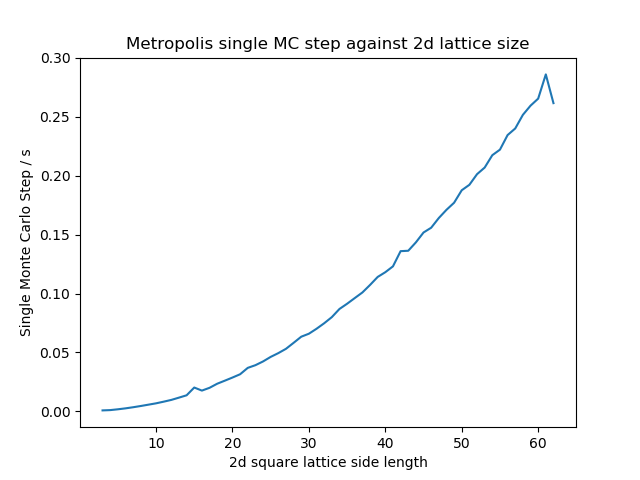
\includegraphics[width=0.7\textwidth]{../figures/metropolis_performance}
	% \ctikzfig{../figures/metropolis_performance}
	\caption{\label{fig:metropolis_performance} Performance of Metropolis algorithm.}
\end{figure}

Time complexity for a single MC step with respect to lattice size $n$ in $d$ dimension is $O(n^{d})$ \ref{fig:metropolis_performance}.

\subsubsection{\label{sec:mc:checker}Checkerboard Algorithm}

\begin{figure}[H] \centering
	% \includegraphics[width=0.5\textwidth]{checkerboard.tikz}
	\ctikzfig{../figures/checkerboard}
	\caption{\label{fig:checkerboard} A 2D Checkerboard example divided into 4 interleaved sub-lattices, sites labeled with a same number are updated simultaneously.}
\end{figure}

\begin{figure}[H] \centering
	% \includegraphics[width=0.5\textwidth]{checkerboard.tikz}
	\ctikzfig{../figures/binary_kernel}
	\caption{\label{fig:binary_kernel} A binary convolution kernel for calculating local interaction energies.}
\end{figure}

Metropolis algorithm is improved by choosing an efficient updating procedure. By dividing into 4 interleaved sub-lattices \ref{fig:checkerboard} then updating a sub-lattice as a whole, we avoid randomizing and reduce the number of function calls. The Checkerboard algorithm was implemented for arbitrary dimension odd sized Ising system. This paper works with odd sized systems without loss of generality. Local interaction energies are computed by convolving spins locally with a binary kernel \ref{fig:binary_kernel} representing local interactions.

\begin{figure}[H] \centering
	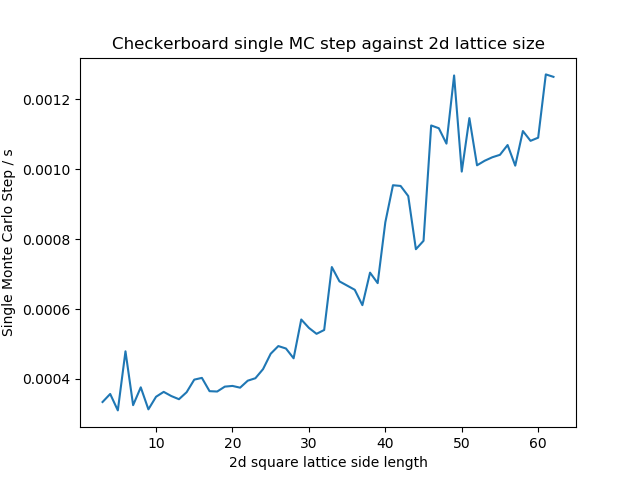
\includegraphics[width=0.65\textwidth]{../figures/checkerboard_performance}
	% \ctikzfig{../figures/checkerboard_performance}
	\caption{\label{fig:checkerboard_performance} Performance of Checkerboard algorithm.}
\end{figure}

\begin{figure}[H] \centering
	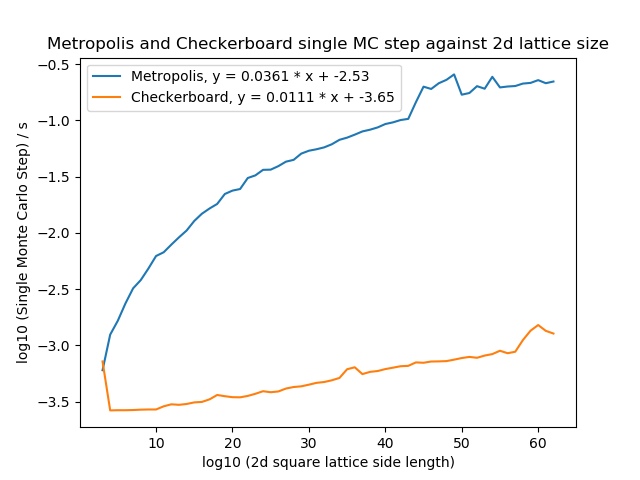
\includegraphics[width=0.7\textwidth]{../figures/comparison_performance}
	% \ctikzfig{../figures/checkerboard_performance}
	\caption{\label{fig:comparison_performance} Performance comparison (log10) between Metropolis and Checkerboard algorithms.}
\end{figure}

Time complexity for a single MC step with lattice size $n$ and $m$ sites being updated simultaneously by numpy vectorized functions is $O(n^{d} / m)$ \ref{fig:checkerboard_performance}. A speedup of more than 100 times is achieved for systems sized between $10$ and $60$ \ref{fig:comparison_performance}, which is the working regime for other sections. This improved computational efficiency enables calculation of larger systems with more accurate error bars in the following sections, especially in simulating hysteresis effect \ref{sec:hysteresis} where quantization errors are undesirable.

\begin{figure}[H] \centering
	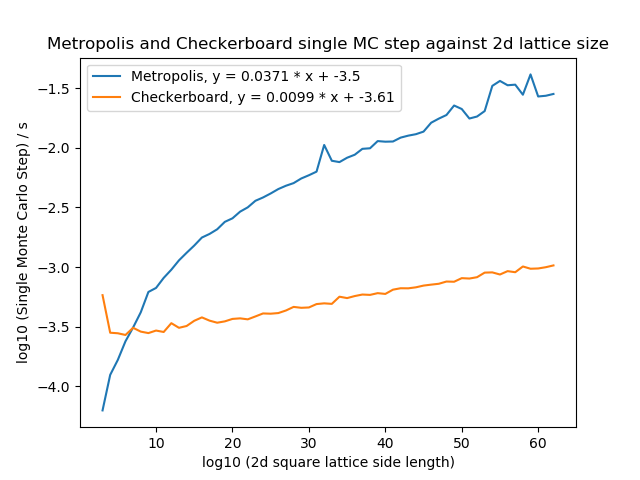
\includegraphics[width=0.7\textwidth]{../figures/metropolis_performance_no_rand}
	% \ctikzfig{../figures/checkerboard_performance}
	\caption{\label{fig:metropolis_performance_no_rand} Performance comparison (log10) between Metropolis (non-random) and Checkerboard algorithms.}
\end{figure}

The Checkerboard algorithm is still more than 100 times faster for systems sized between 30 and 60 \ref{fig:metropolis_performance_no_rand} compared with non-random Metropolis.

\subsection{\label{sec:method:error}Error Estimation}

Errors are deduced from repeated measurements. Ising model produces correlated data, therefore Jackknife algorithm is used as opposed to Bootstrap algorithm for non-trivial statistics, e.g. Binder's Cumulent. Standard deviation is used when the desired statistics is mean.

\section{\label{sec:equi_time}Equilibrium Time}
A Gaussian clustering algorithm in total magnetization phase-space determines time taken to reach equilibrium state from a random initial state, where each site is equally likely to be spin up or down. Assuming system moves to an equilibrium state eventually, any long enough simulation will have the minority cluster size corresponding to the equilibrium time. This algorithm is applicable to all MC processes where the phase space is localized in equilibrium state.

We will test the algorithm validity and plot equilibrium time against temperature on a 41 by 41 system. 





\subsection{\label{sec:equi_time:method}Methods}

\begin{algorithm}[H]
	\setstretch{1.35} 
	\caption{Equilibrium state detection}
	\label{alg:equilibrium_detection}
	\begin{algorithmic}
		\REQUIRE ~~\\
		
		Long enough (5 times longer than the correlation time) simulated total magnetization time series;\\
		\label{code:equi_detect:long_simulation}
		
		\ENSURE ~~\\
		% Demean magnetization time series and normalize using mean magnitude;
		Cluster total magnetization phase space into 2 Gaussian clusters;\\
		\label{code:equi_detect:gaussian_cluster}
		If cluster sizes differ by more than half of the simulation time, the minority cluster size is returned as the time taken to reach equilibrium;\\
		Else either system started in or has not reached equilibrium and a longer simulation time may be needed, and returns 0 as equilibrium time by default.
		\label{code:equi_detect:size_difference}
	\end{algorithmic}
\end{algorithm}

Notice that a default equilibrium time 0 is returned when the algorithm fails to detect any equilibrium state.

\subsection{\label{sec:equi_time:results}Results}

\begin{figure}[H] \centering
	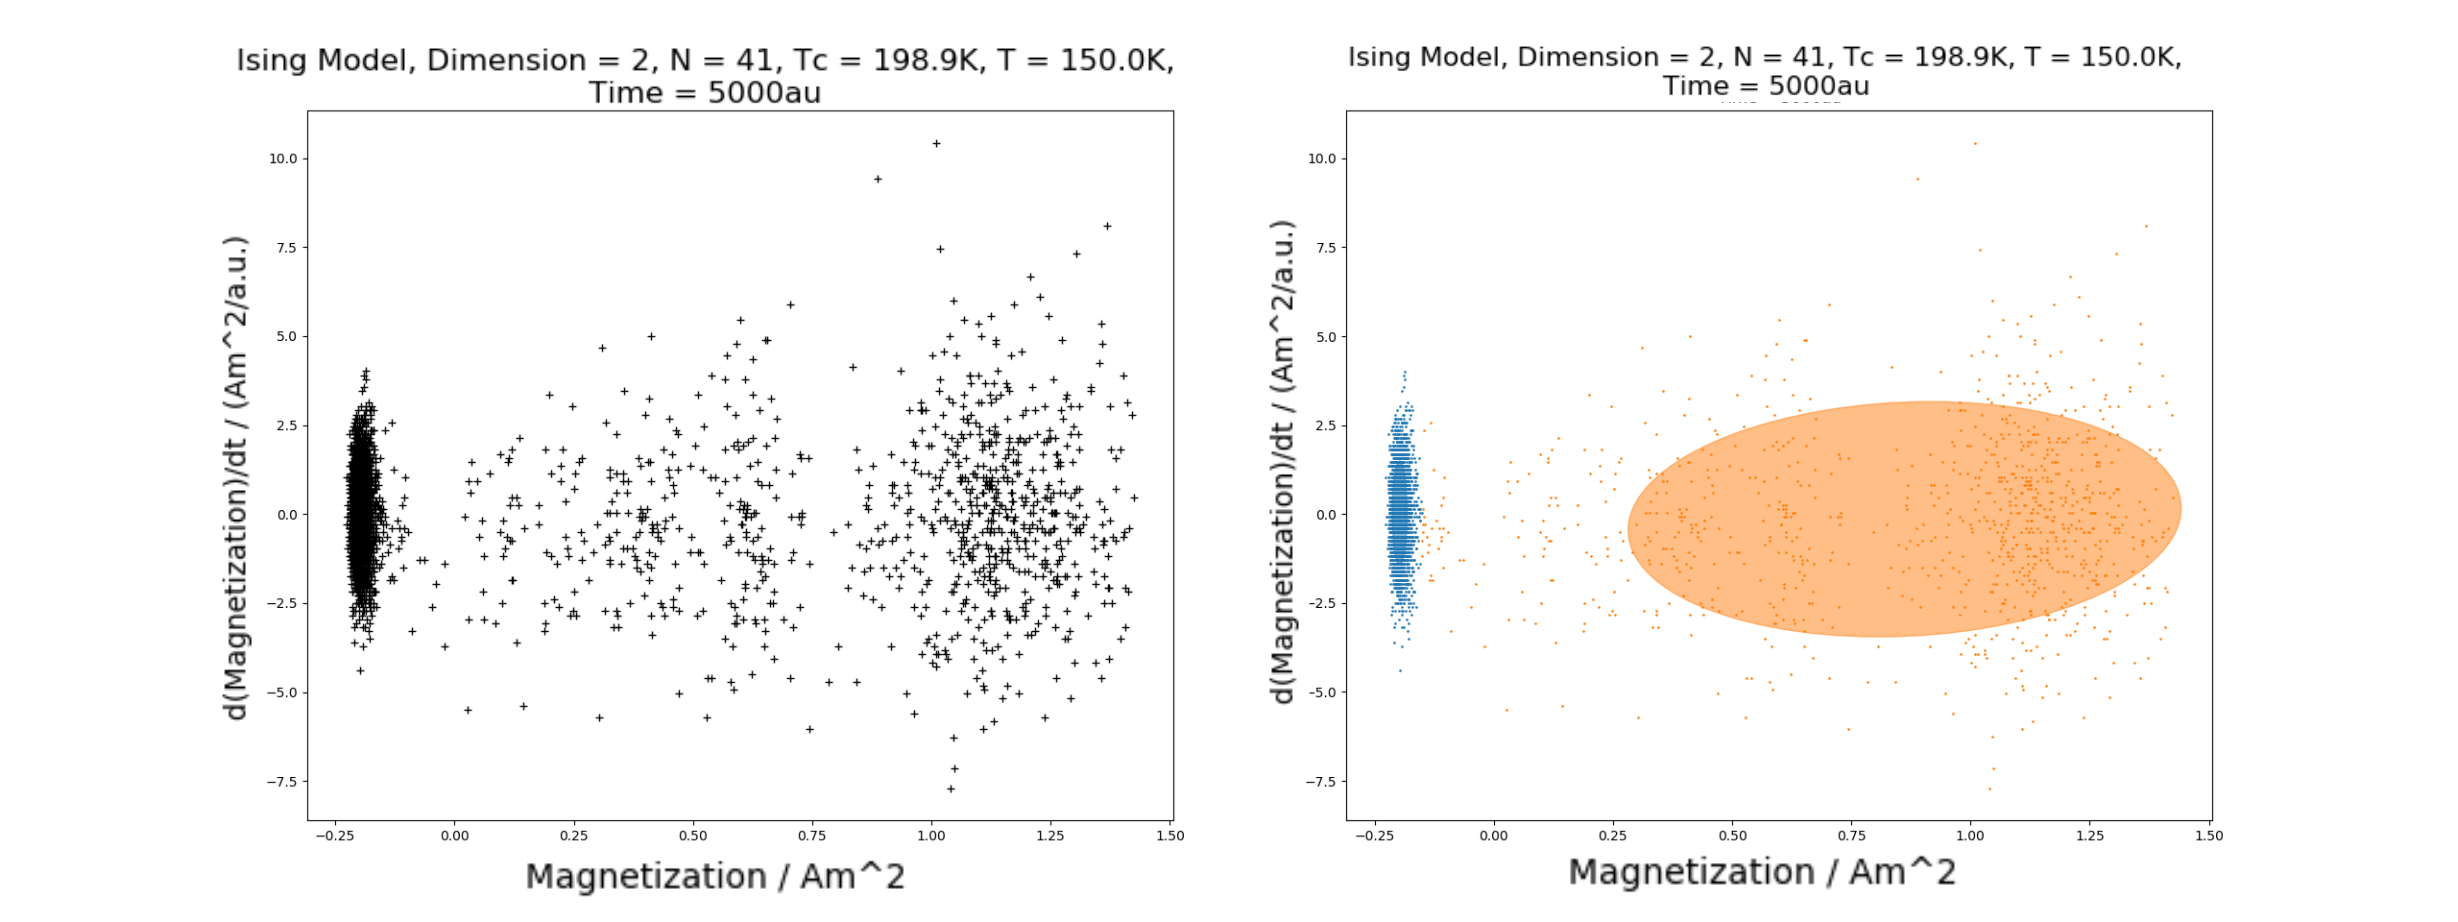
\includegraphics[width=1.1\textwidth]{../figures/equi_time_phasespace}
	% \ctikzfig{../figures/checkerboard_performance}
	\caption{\label{fig:equi_time_phasespace} Magnetization phase space clustering.}
\end{figure}

Clustering on a system below Curie temperature \ref{fig:equi_time_phasespace} shows a densely populated equilibrium state cluster in blue, with minority cluster in orange representing other intermediate states in reaching equilibrium.

\begin{figure}[H] \centering
	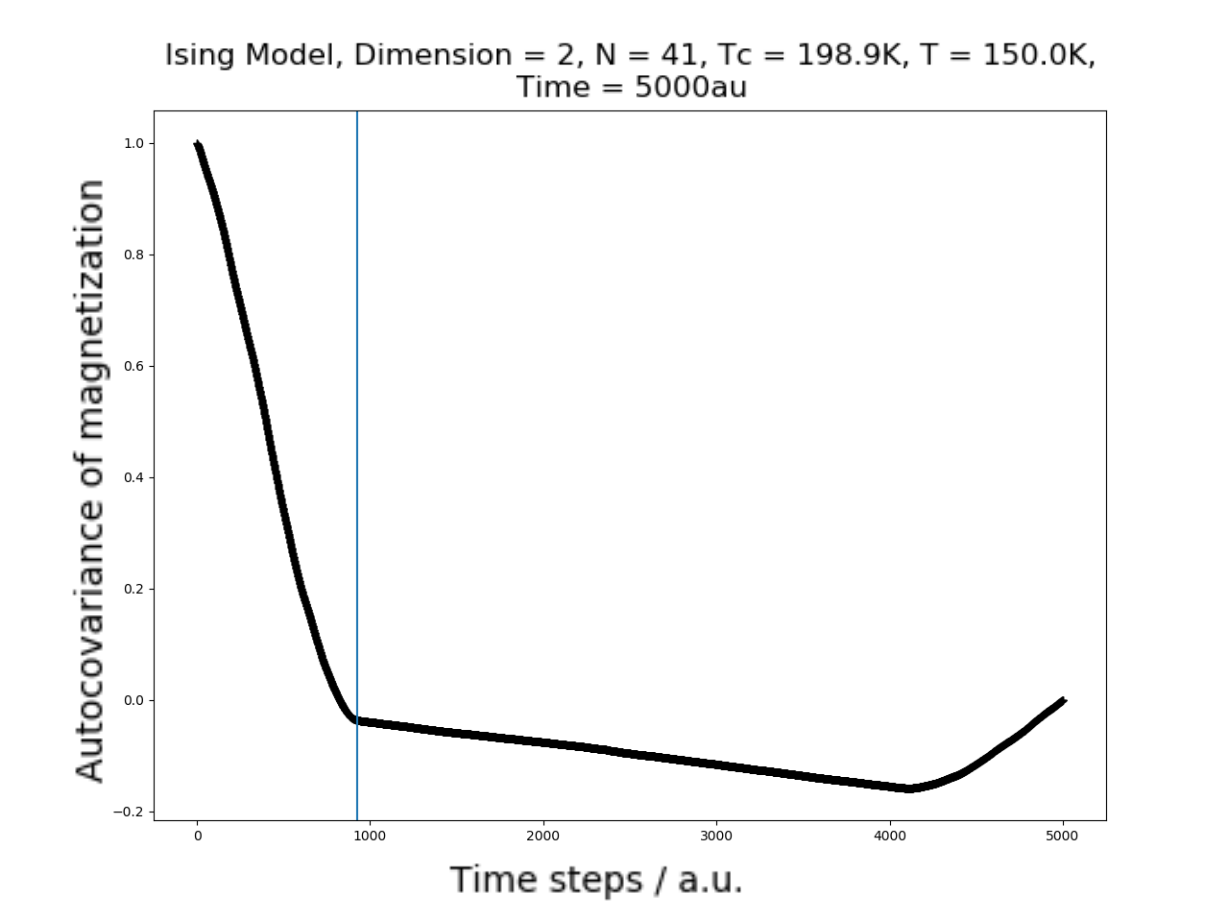
\includegraphics[width=0.7\textwidth]{../figures/equi_time_autocovariance}
	% \ctikzfig{../figures/checkerboard_performance}
	\caption{\label{fig:equi_time_autocovariance} Equilibrium time (blue line) on auto-covariance against time graph.}
\end{figure}

\begin{figure}[H] \centering
	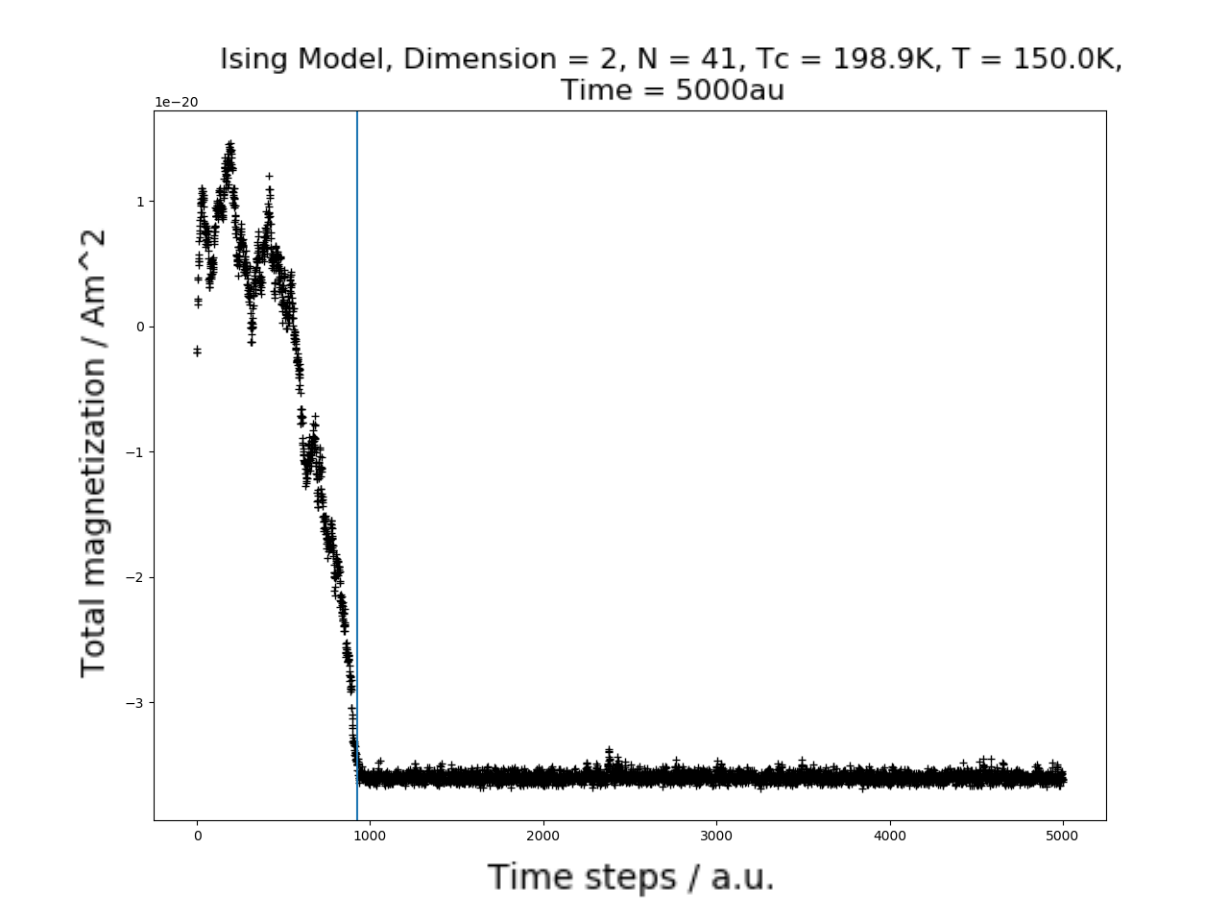
\includegraphics[width=0.7\textwidth]{../figures/equi_time_magnetization}
	% \ctikzfig{../figures/checkerboard_performance}
	\caption{\label{fig:equi_time_magnetization} Equilibrium time (blue line) on magnetization against time graph.}
\end{figure}

\begin{figure}[H] \centering
	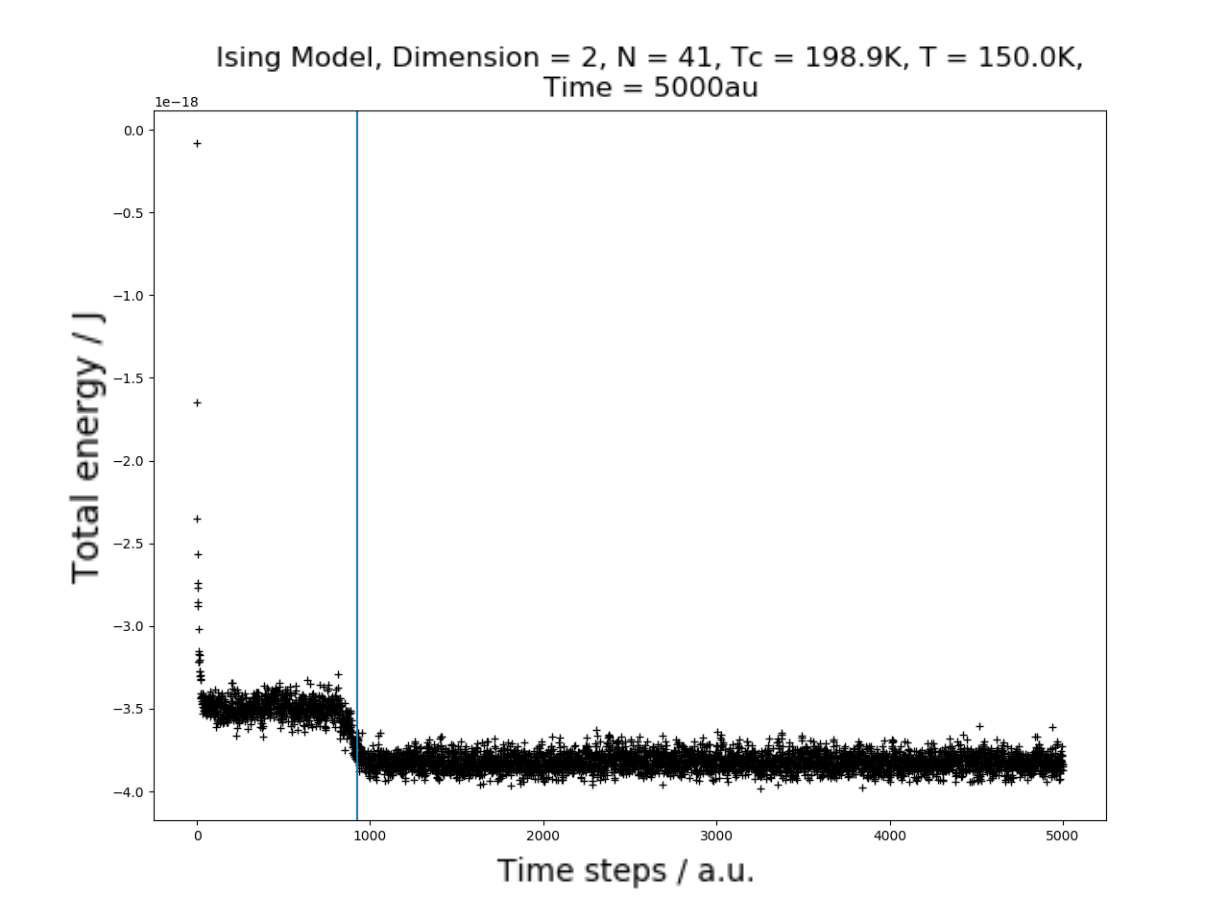
\includegraphics[width=0.75\textwidth]{../figures/equi_time_total_energy}
	% \ctikzfig{../figures/checkerboard_performance}
	\caption{\label{fig:equi_time_total_energy} Equilibrium time (blue line) on total energy against time graph.}
\end{figure}

From \ref{fig:equi_time_autocovariance}, \ref{fig:equi_time_magnetization} and \ref{fig:equi_time_total_energy} the estimation of equilibrium time passes the sanity check by noticing the overlapping of the blue line (estimation) and the start of the equilibrium state.

\begin{figure}[H] \centering
	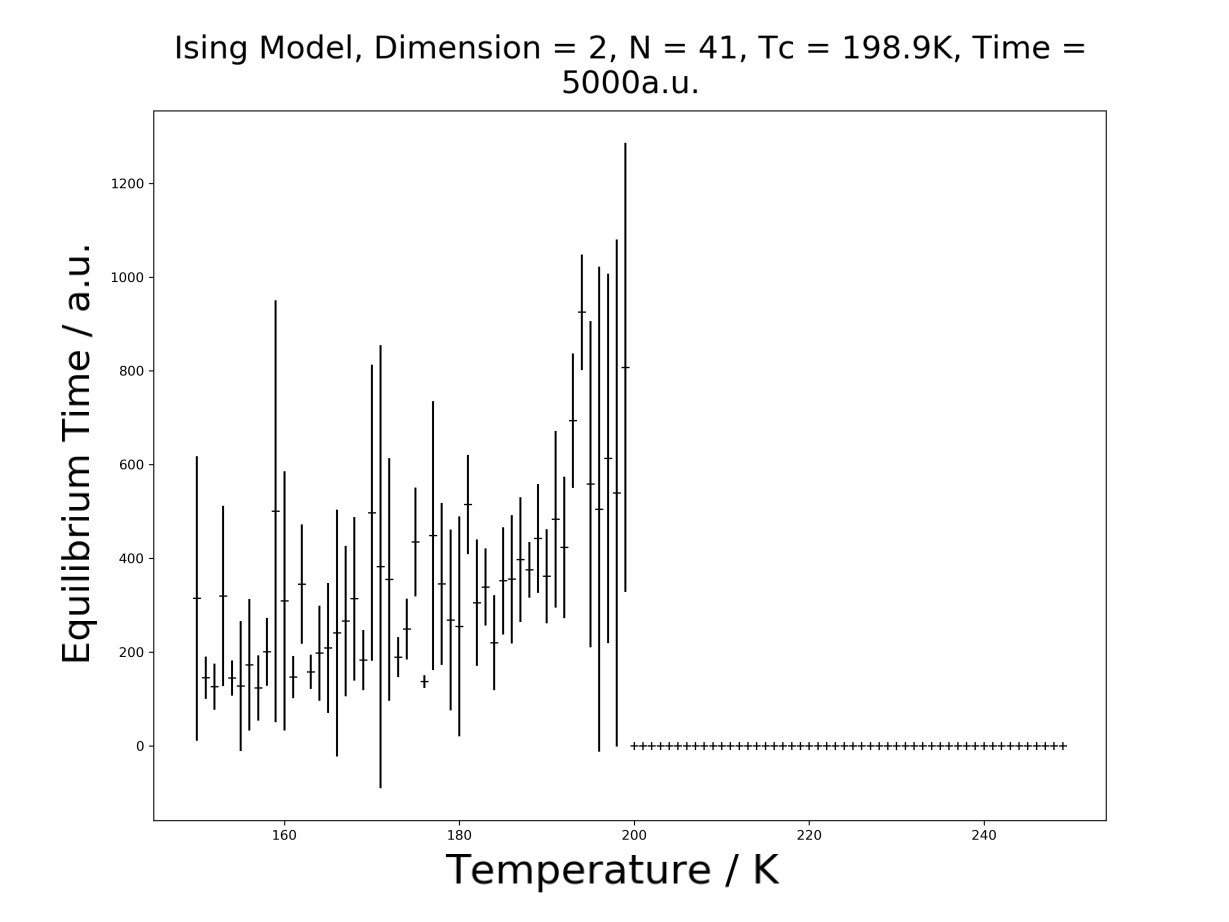
\includegraphics[width=0.75\textwidth]{../figures/equiliibrium_times_vs_temperature}
	% \ctikzfig{../figures/checkerboard_performance}
	\caption{\label{fig:equiliibrium_times_vs_temperature} Equilibrium time against temperature.}
\end{figure}

Time taken to reach equilibrium depends on the difference between initial state and the equilibrium state, and the correlation time. In the low temperature regime with a short correlation time, the initial state is a hot state (high energy) and far from the equilibrium state. Near and below the Curie temperature with a long correlation length, the system is in a cold state (low energy) and close to the equilibrium state. We observe a growing equilibrium time in temperature below the Curie temperature, implying equilibrium time grows with and is dominated by correlation time.

Above the Curie temperature, system is already in the equilibrium state and equilibrium time is zero.

\section{\label{sec:level1}Correlation Time}

Correlation time is the amount of time the system needs to evolve such that the initial state becomes irrelevant in the case of pure thermal fluctuations. When averaging to measure any physical quantities, we must average over more than at least 2 correlation time to get the result to reduce random error. We will study the correlation time for systems of sizes 11, 15 and 19, focusing on near Curie temperature behaviour.

\subsection{\label{sec:level2}Methods}
\begin{algorithm}[H]
	\setstretch{1.35} 
	\caption{Auto-correlation time}
	\label{alg:auto_correlation}
	\begin{algorithmic}
		\REQUIRE ~~\\
		
		All sites' spins initialized;\\
		\label{code:auto_correlation:initialize}
		
		\ENSURE ~~\\
		
		Evolve the system for more than 5 times of the correlation time;\\
		\label{code:auto_correlation:evolve}
		Determine and discard non-equilibrium evolution section of the time series;\\
		\label{code:auto_correlation:discard_non_equi}
		Compute the auto-correlation for the remaining magnetization time series, normalized by auto-correlation at $\Delta t = 0$;\\
		\label{code:auto_correlation:normalized_auto_correlation}
		Identify time taken for normalized auto-correlation to drop below $1/e$ as the correlation time;\\
		\label{code:auto_correlation:below_1/e_time}
	\end{algorithmic}
\end{algorithm}

Single measurement was carried out using \ref{alg:auto_correlation}, and repeated measurements were taken to measure the error.

\subsection{\label{sec:level2}Results}

\begin{figure}[H] \centering
	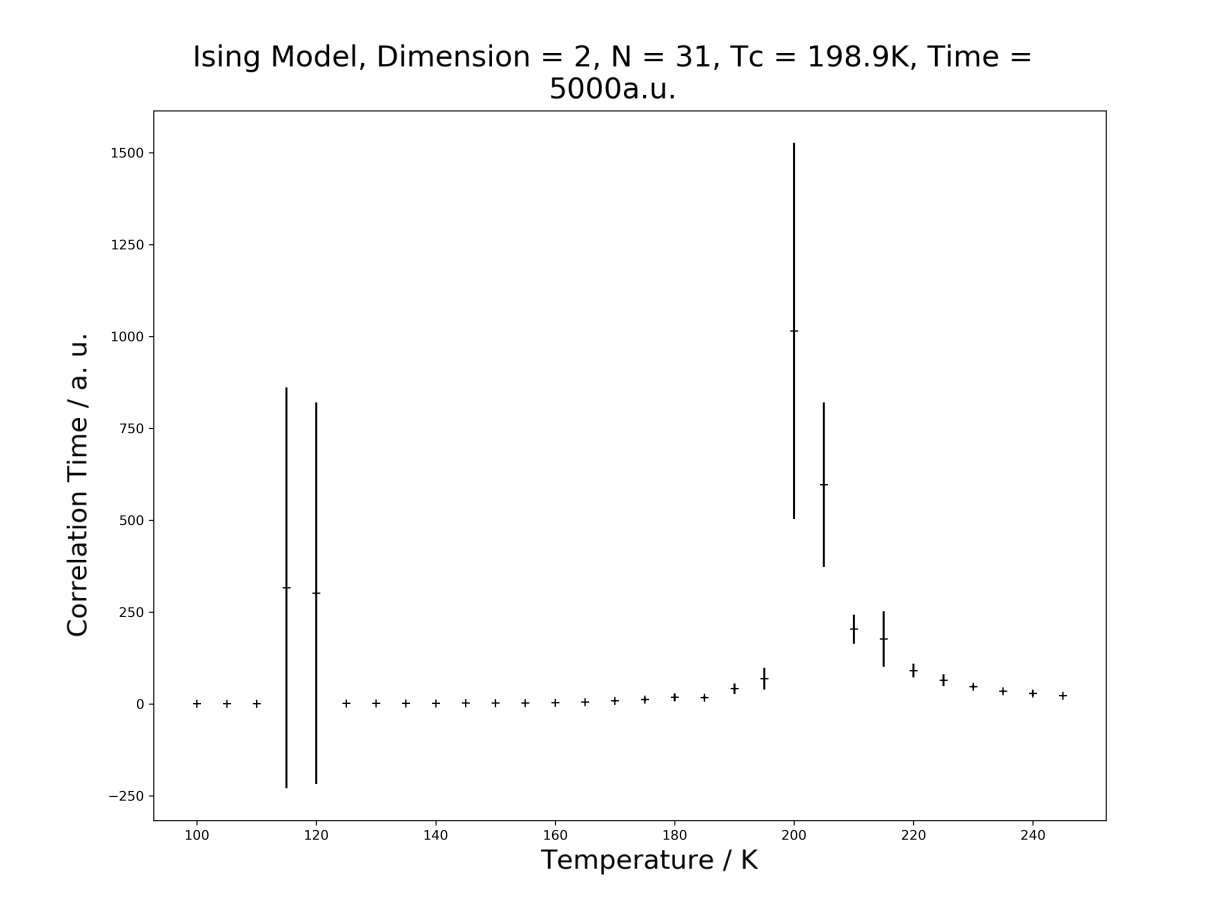
\includegraphics[width=0.7\textwidth]{../figures/auto_corre_scan}
	% \ctikzfig{../figures/checkerboard_performance}
	\caption{\label{fig:auto_corre_scan} Correlation time against temperature over ordered and disordered phases.}
\end{figure}

The singular point in correlation time is around $200K$. We zoom in onto that section for systems of size 11, 15 and 19.

\begin{figure}[H] \centering
	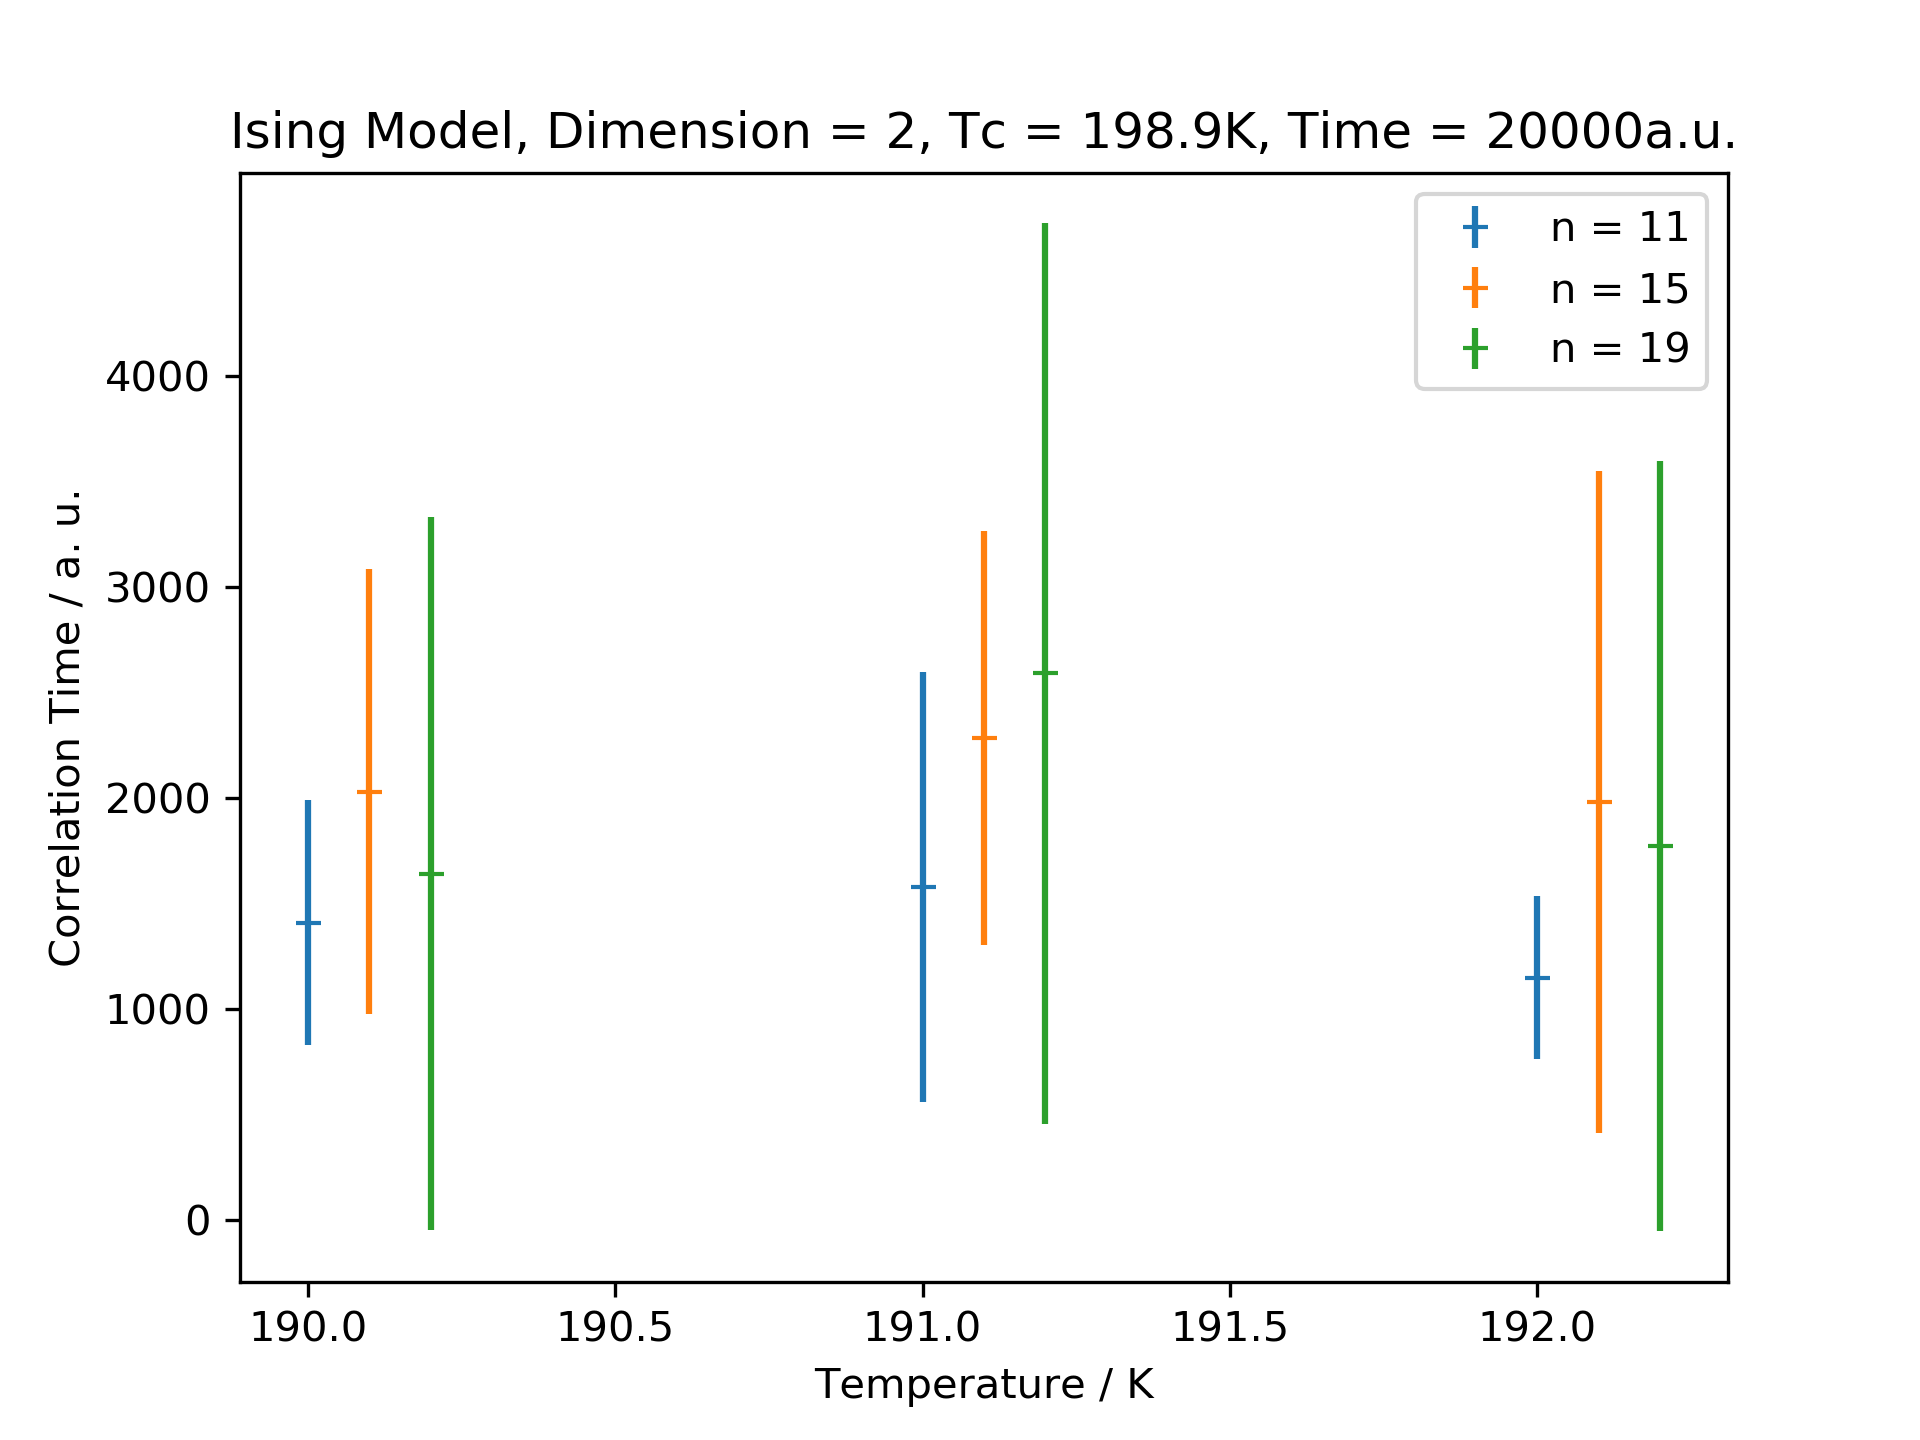
\includegraphics[width=0.7\textwidth]{../figures/mag_mag_different_size}
	% \ctikzfig{../figures/checkerboard_performance}
	\caption{\label{fig:mag_mag_different_size} Correlation time for systems of different sizes around the Curie point.}
\end{figure}

Correlation time increases from around 1000 to 2000 as the system size increases \ref{fig:mag_mag_different_size}. Curie point is located around the highest correlation time, at $191K$. This implies that at least 10000 MC steps is needed for systems sized between 11 and 21 near the Curie temperature. It is allowed to run for less MC steps for off Curie point simulations. 

Calculating correlation time is longer than measuring most physical quantities, we effectively choose an upper bound (e.g. 10000 MC steps) and does not calculate the correlation time every time when making measurements.

\section{\label{sec:level1}Equilibrium Magnetization}

We will study the temperature dependence of the equilibrium magnetization for systems of size 31, focusing on near Curie temperature behaviour.

\subsection{\label{sec:level2}Method}

\begin{algorithm}[H]
	\setstretch{1.35} 
	\caption{Equilibrium magnetization}
	\label{alg:equi_mag}
	\begin{algorithmic}
		\REQUIRE ~~\\
		
		All sites' spins initialized;\\
		\label{code:equi_mag:initialize}
		
		\ENSURE ~~\\
		
		Evolve the system for more than 10 times of the correlation time;\\
		\label{code:equi_mag:evolve}
		Determine and discard non-equilibrium evolution time series;\\
		\label{code:equi_mag:discard_non_equi}
		Return mean of the remaining magnetization time series.
	\end{algorithmic}
\end{algorithm}

Single equilibrium magnetization measurement is carried out using \ref{alg:equi_mag}. Repeated measurements gives an estimate for the error.

\subsection{\label{sec:level2}Result}

Scanning the whole temperature domain helps find the phase transition point of the order parameter.

\begin{figure}[H] \centering
	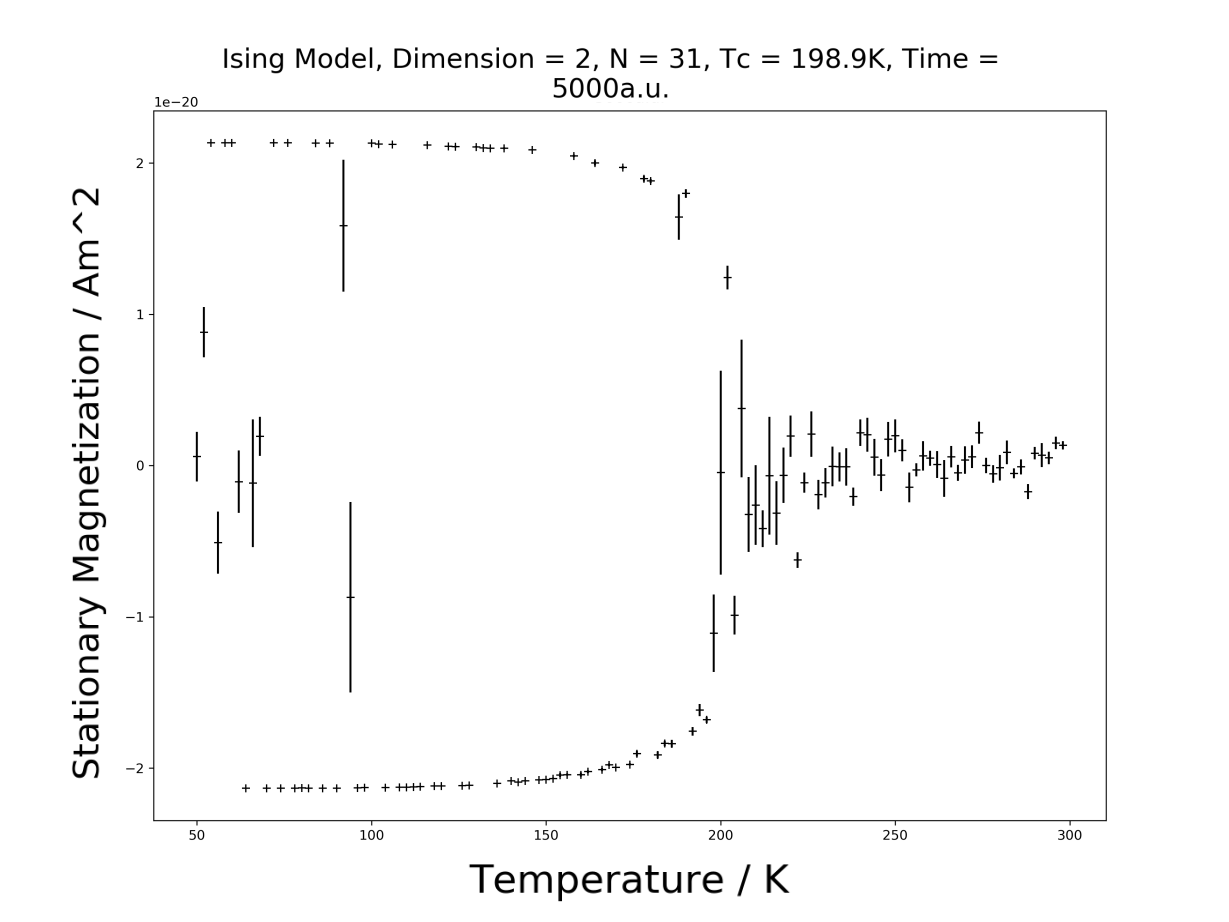
\includegraphics[width=0.7\textwidth]{../figures/mag_mag_31_50_2_125}
	% \ctikzfig{../figures/mag_mag_200_80_0.5}
	\caption{\label{fig:mag_mag_31_50_2_125} Equilibrium magnetization for ordered and disordered phases.}
\end{figure}

High temperature regime exhibits disordered phase while low temperature regime exhibits ordered phase \ref{fig:mag_mag_31_50_2_125}. 8 outliers near zero magnetization at low temperature are due to system being unable to move out of local energy minima by insufficient thermal fluctuations. We notice that thermal fluctuations is strongest around the theoretical Curie temperature $T_C=198.9K$ \ref{eq:curie_temp}.

A phase transition is observed above 200K. We zoom in on 200K to 250K region to study the phase transition behaviour.

\begin{figure}[H] \centering
	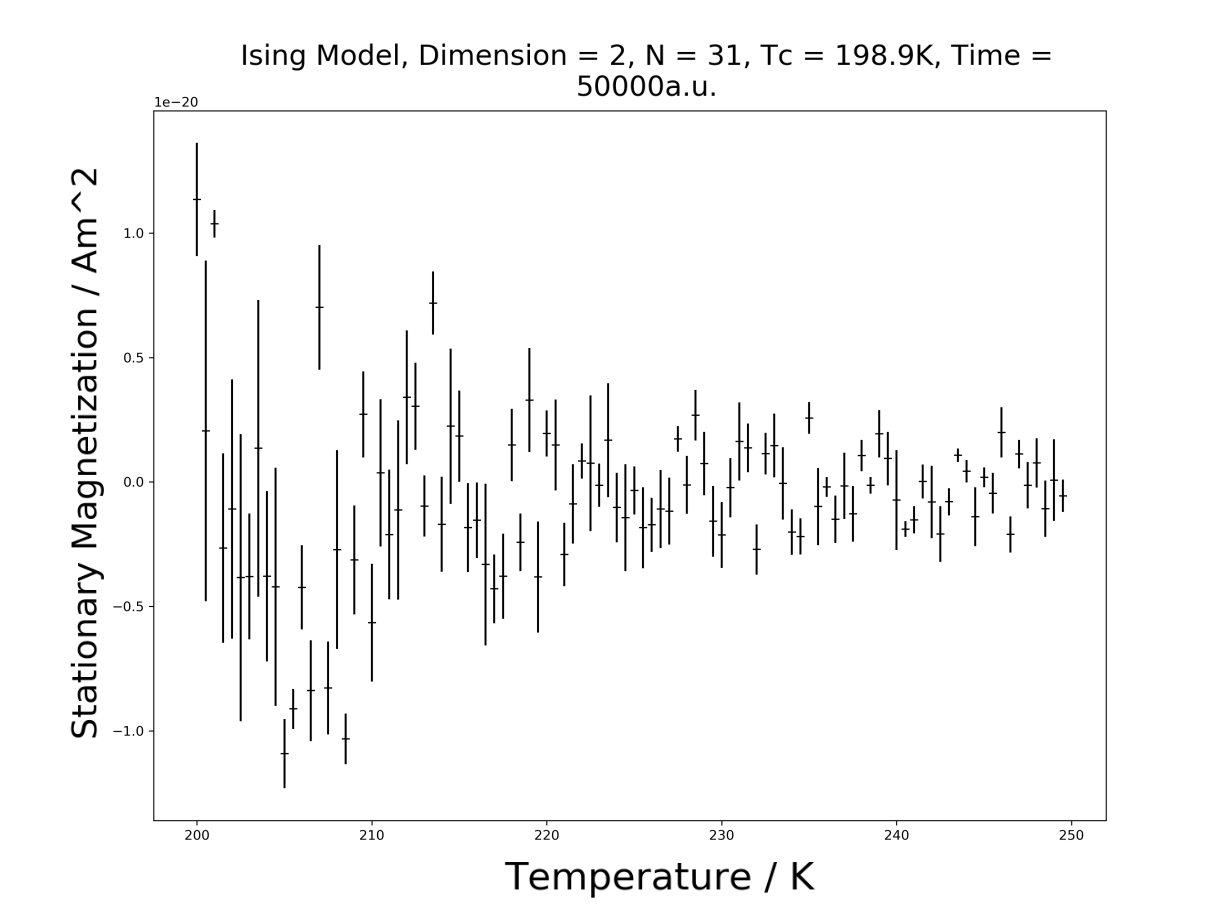
\includegraphics[width=0.7\textwidth]{../figures/mag_mag_31_200_0.5_100}
	% \ctikzfig{../figures/mag_mag_200_80_0.5}
	\caption{\label{fig:mag_mag_31_200_0.5_100} Equilibrium magnetization with Curie point details.}
\end{figure}

A transition from ordered phase into disordered phase is observed around 228K. Anomalously low thermal fluctuation was observed for the equilibrium magnetization around the phase transition point. This is possibly due to the finite size effect displacing the phase transition point of the order parameter from the singularity point of the correlation time.

\section{\label{sec:level1}Finite Size Scaling of Curie Temperature from Specific Heat Capacity}

We measure the singular point for specific heat capacity, and non-linearly fit the data using scipy.optimize.curve\_fit according to \ref{eq:finite_size_scaling} to obtain $T(\infty)$ for the finite size scaling.
% , $a$ and $\nu$ 

\subsection{\label{sec:level2}Method}

\begin{algorithm}[H]
	\setstretch{1.35} 
	\caption{Specific Heat Capacity}
	\label{alg:spec_heat}
	\begin{algorithmic}
		\REQUIRE ~~\\
		
		Initialize all spins;\\
		\label{code:equi_mag:initialize}
		
		\ENSURE ~~\\
		Evolve the system for more than 5 times of the correlation time;\\
		\label{code:equi_mag:evolve}
		Compute $C = \frac{{\sigma_E}^2}{k_B T^2}$ \ref{eq:spec_heat} as the specific heat.
		
	\end{algorithmic}
\end{algorithm}

\begin{algorithm}[H]
	\setstretch{1.35} 
	\caption{Determine Curie Temperature for given system size}
	\label{alg:Curie_point}
	\begin{algorithmic}
		\REQUIRE ~~\\
		
		Determine the range to look for Curie temperature;\\
		Determine an array of points to explore within that range, spaced $\Delta T$.\\
		Run the system for 10 times as long as the longest correlation time present among the points in the array.
		\label{code:equi_mag:initialize}
		
		\ENSURE ~~\\
		
		Compute Specific heat capacity for all points in the array;\\
		\label{code:equi_mag:evolve}
		Point with the largest specific heat capacity is the predicted Curie point, where the error is over-estimated as $\Delta T$.\\
	\end{algorithmic}
\end{algorithm}

\subsection{\label{sec:level2}Result}

\begin{figure}[H] \centering
	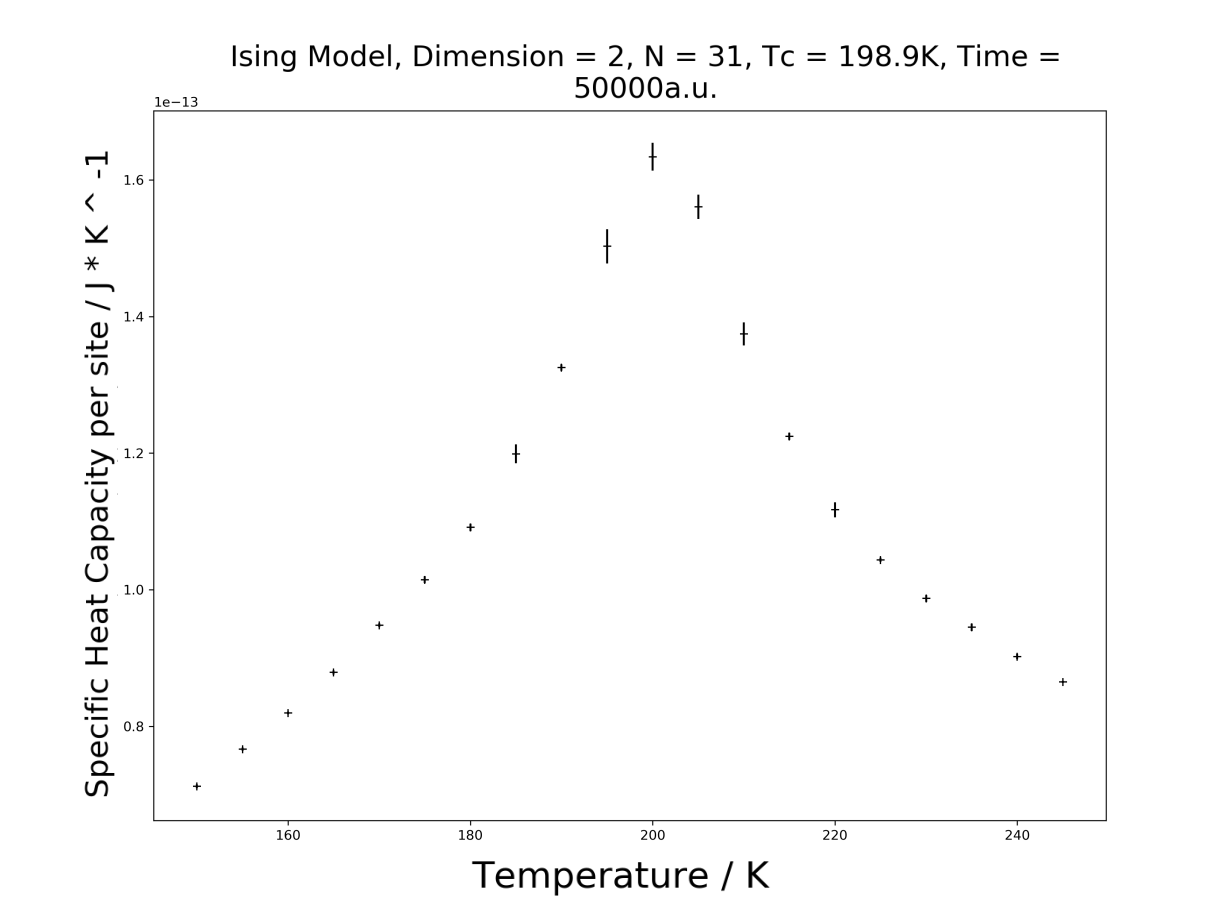
\includegraphics[width=0.7\textwidth]{../figures/specific_heat_scan}
	% \ctikzfig{../figures/mag_mag_200_80_0.5}
	\caption{\label{fig:specific_heat_scan} Specific heat capacity for 31 by 31 system.}
\end{figure}

By scanning the relevant temperature range, the Curie point is located around $200K$. This reduces the searching domain size for $T_C$. We proceed to calculate the Curie point within $190K$ to $210K$.

\begin{figure}[H] \centering
	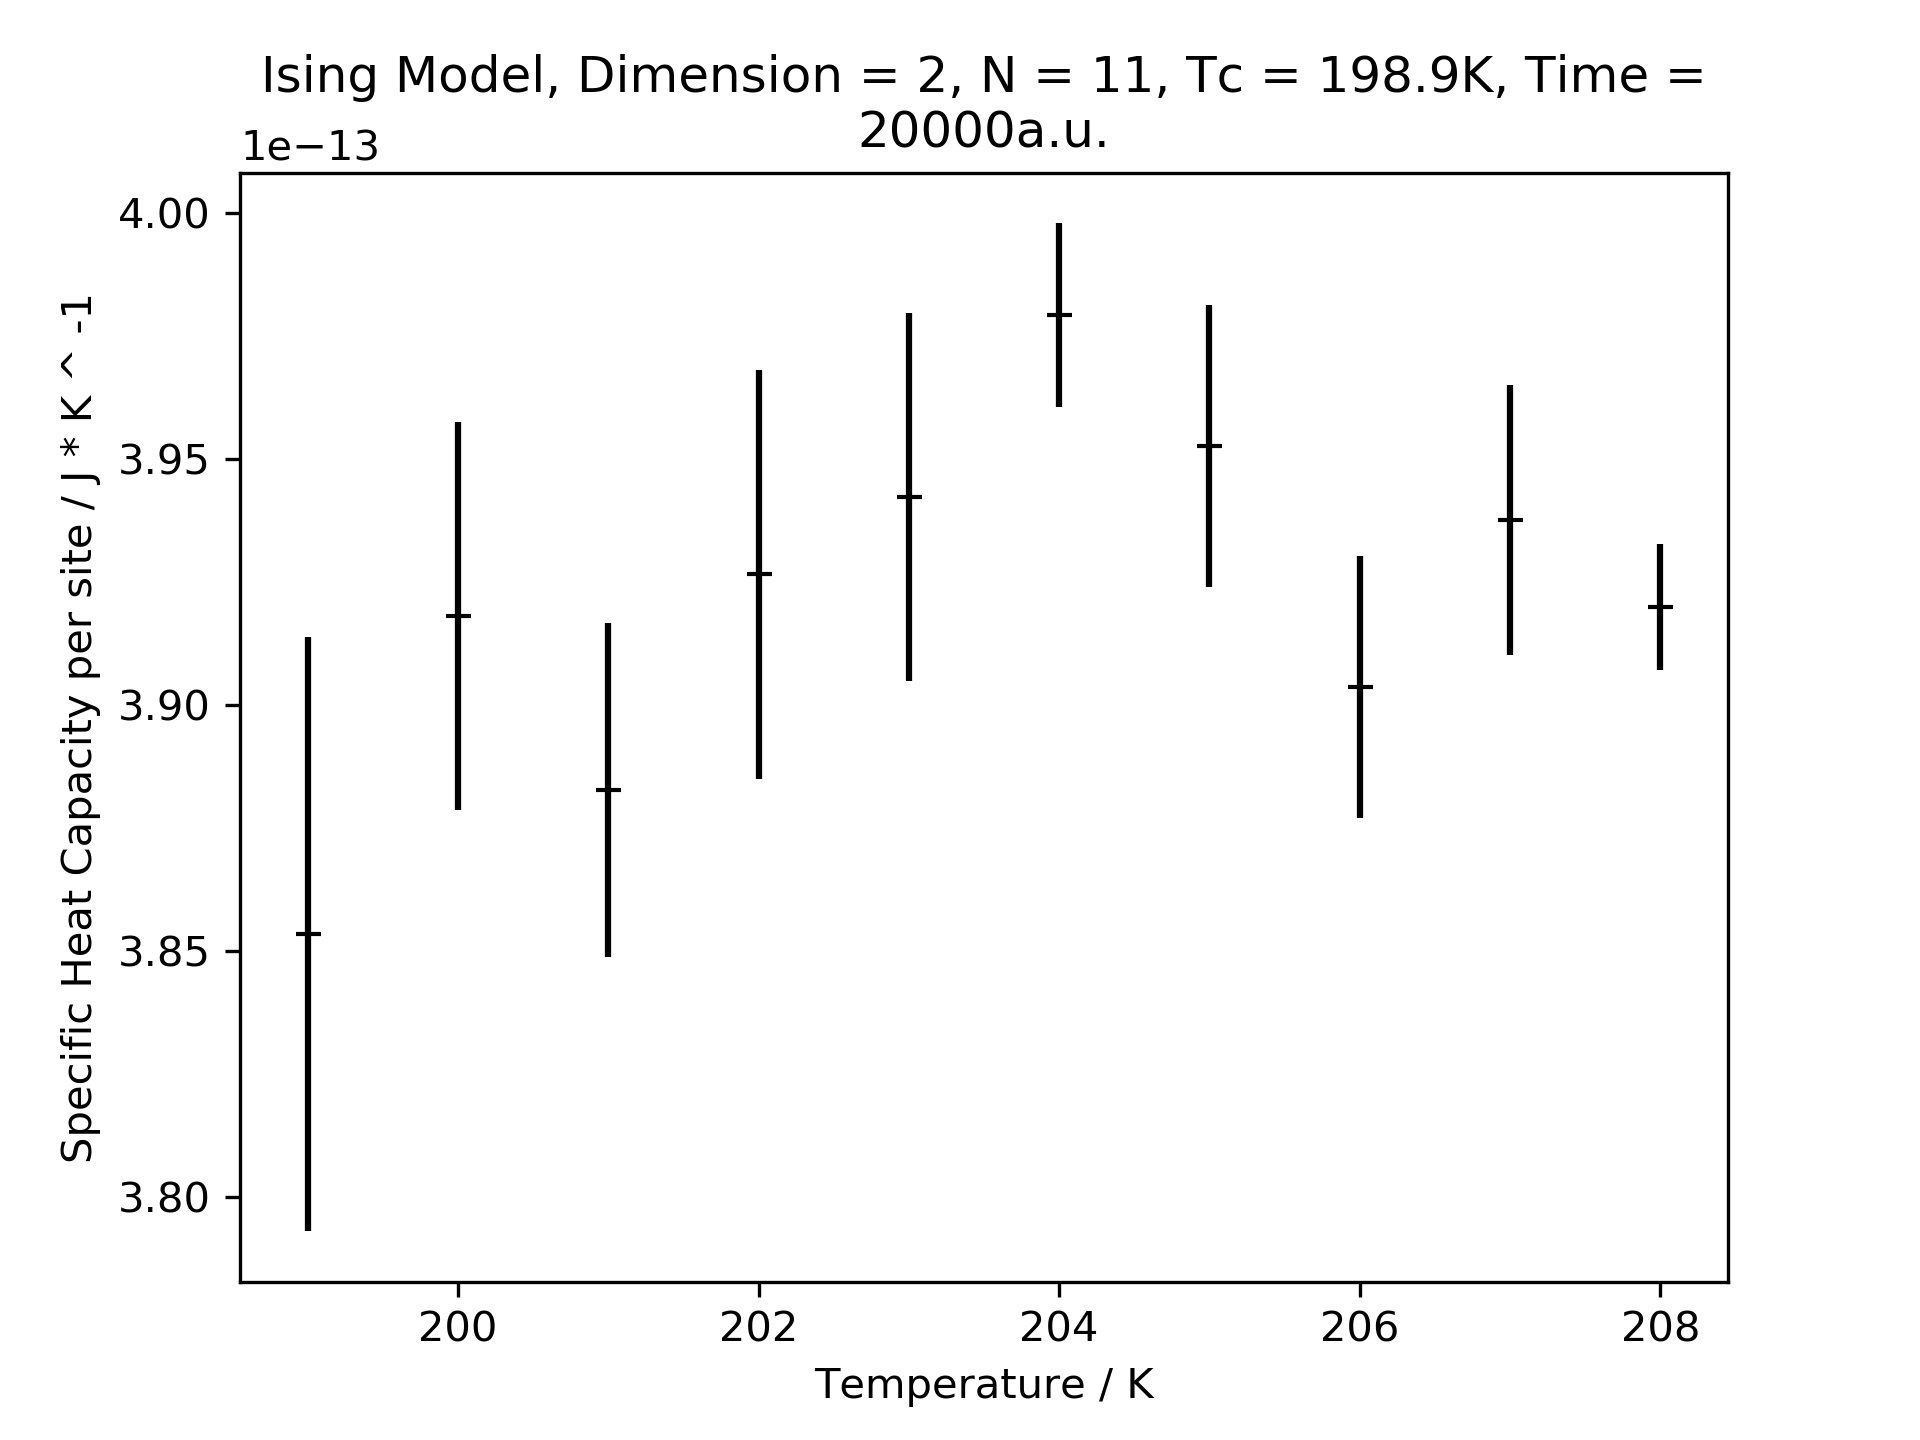
\includegraphics[width=0.7\textwidth]{../figures/size11scan}
	% \ctikzfig{../figures/mag_mag_200_80_0.5}
	\caption{\label{fig:size11scan} Specific heat capacity for 11 by 11 system near Curie point.}
\end{figure}

\begin{figure}[H] \centering
	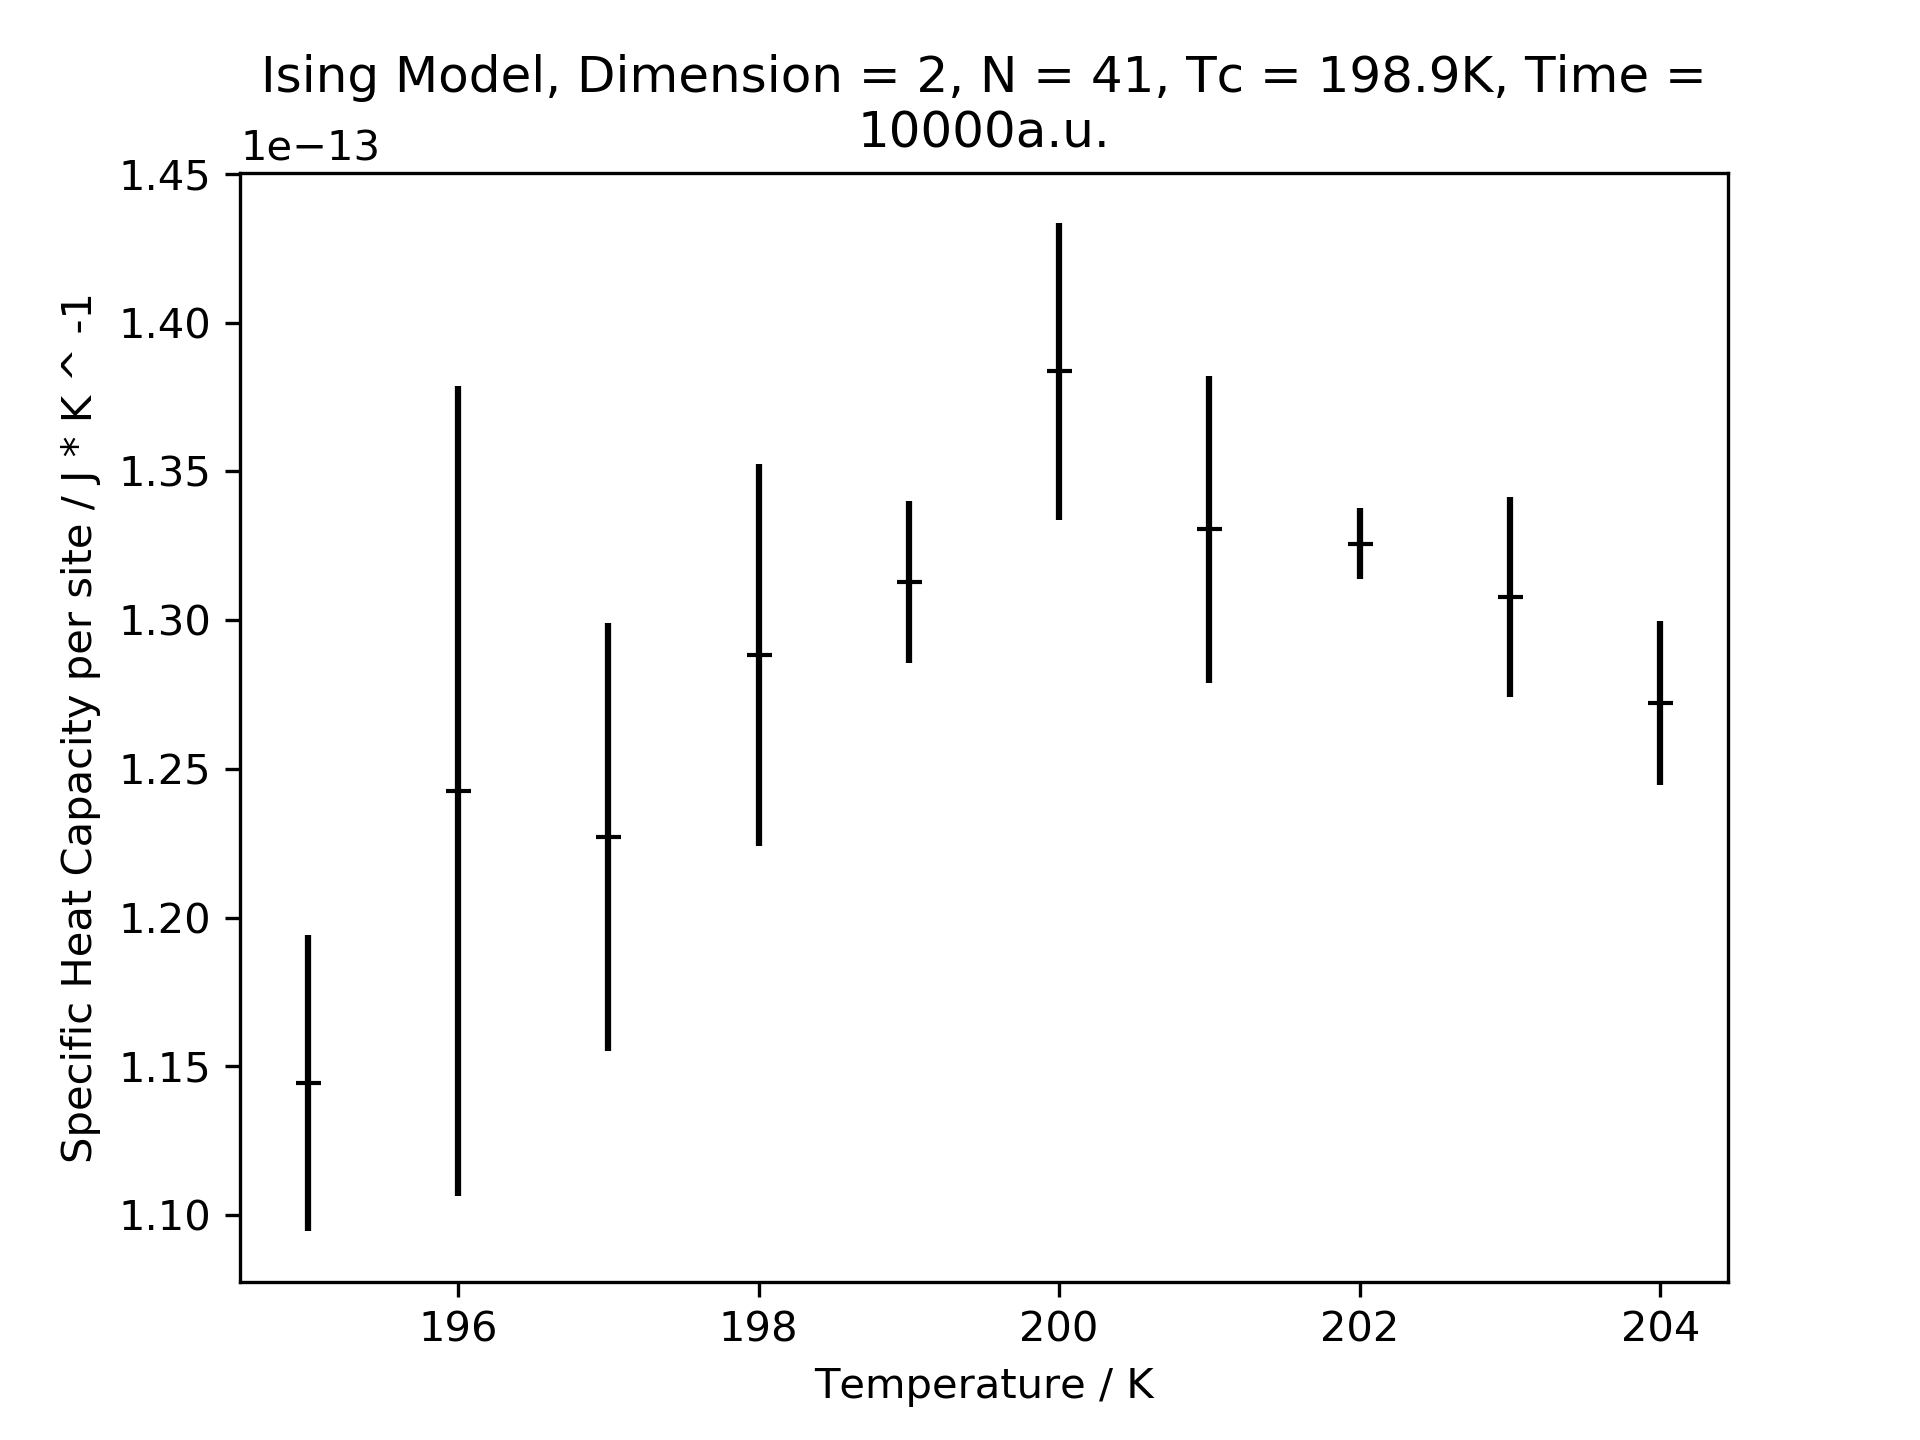
\includegraphics[width=0.7\textwidth]{../figures/size41scan}
	% \ctikzfig{../figures/mag_mag_200_80_0.5}
	\caption{\label{fig:size41scan} Specific heat capacity for 41 by 41 system near Curie point.}
\end{figure}

Curie temperatures for systems between size 41 and 11 lie between $199K$ \ref{fig:size41scan} and $206K$ \ref{fig:size11scan}. We proceed to plot Curie temperatures against sizes between 11 and 41.


\begin{figure}[H] \centering
	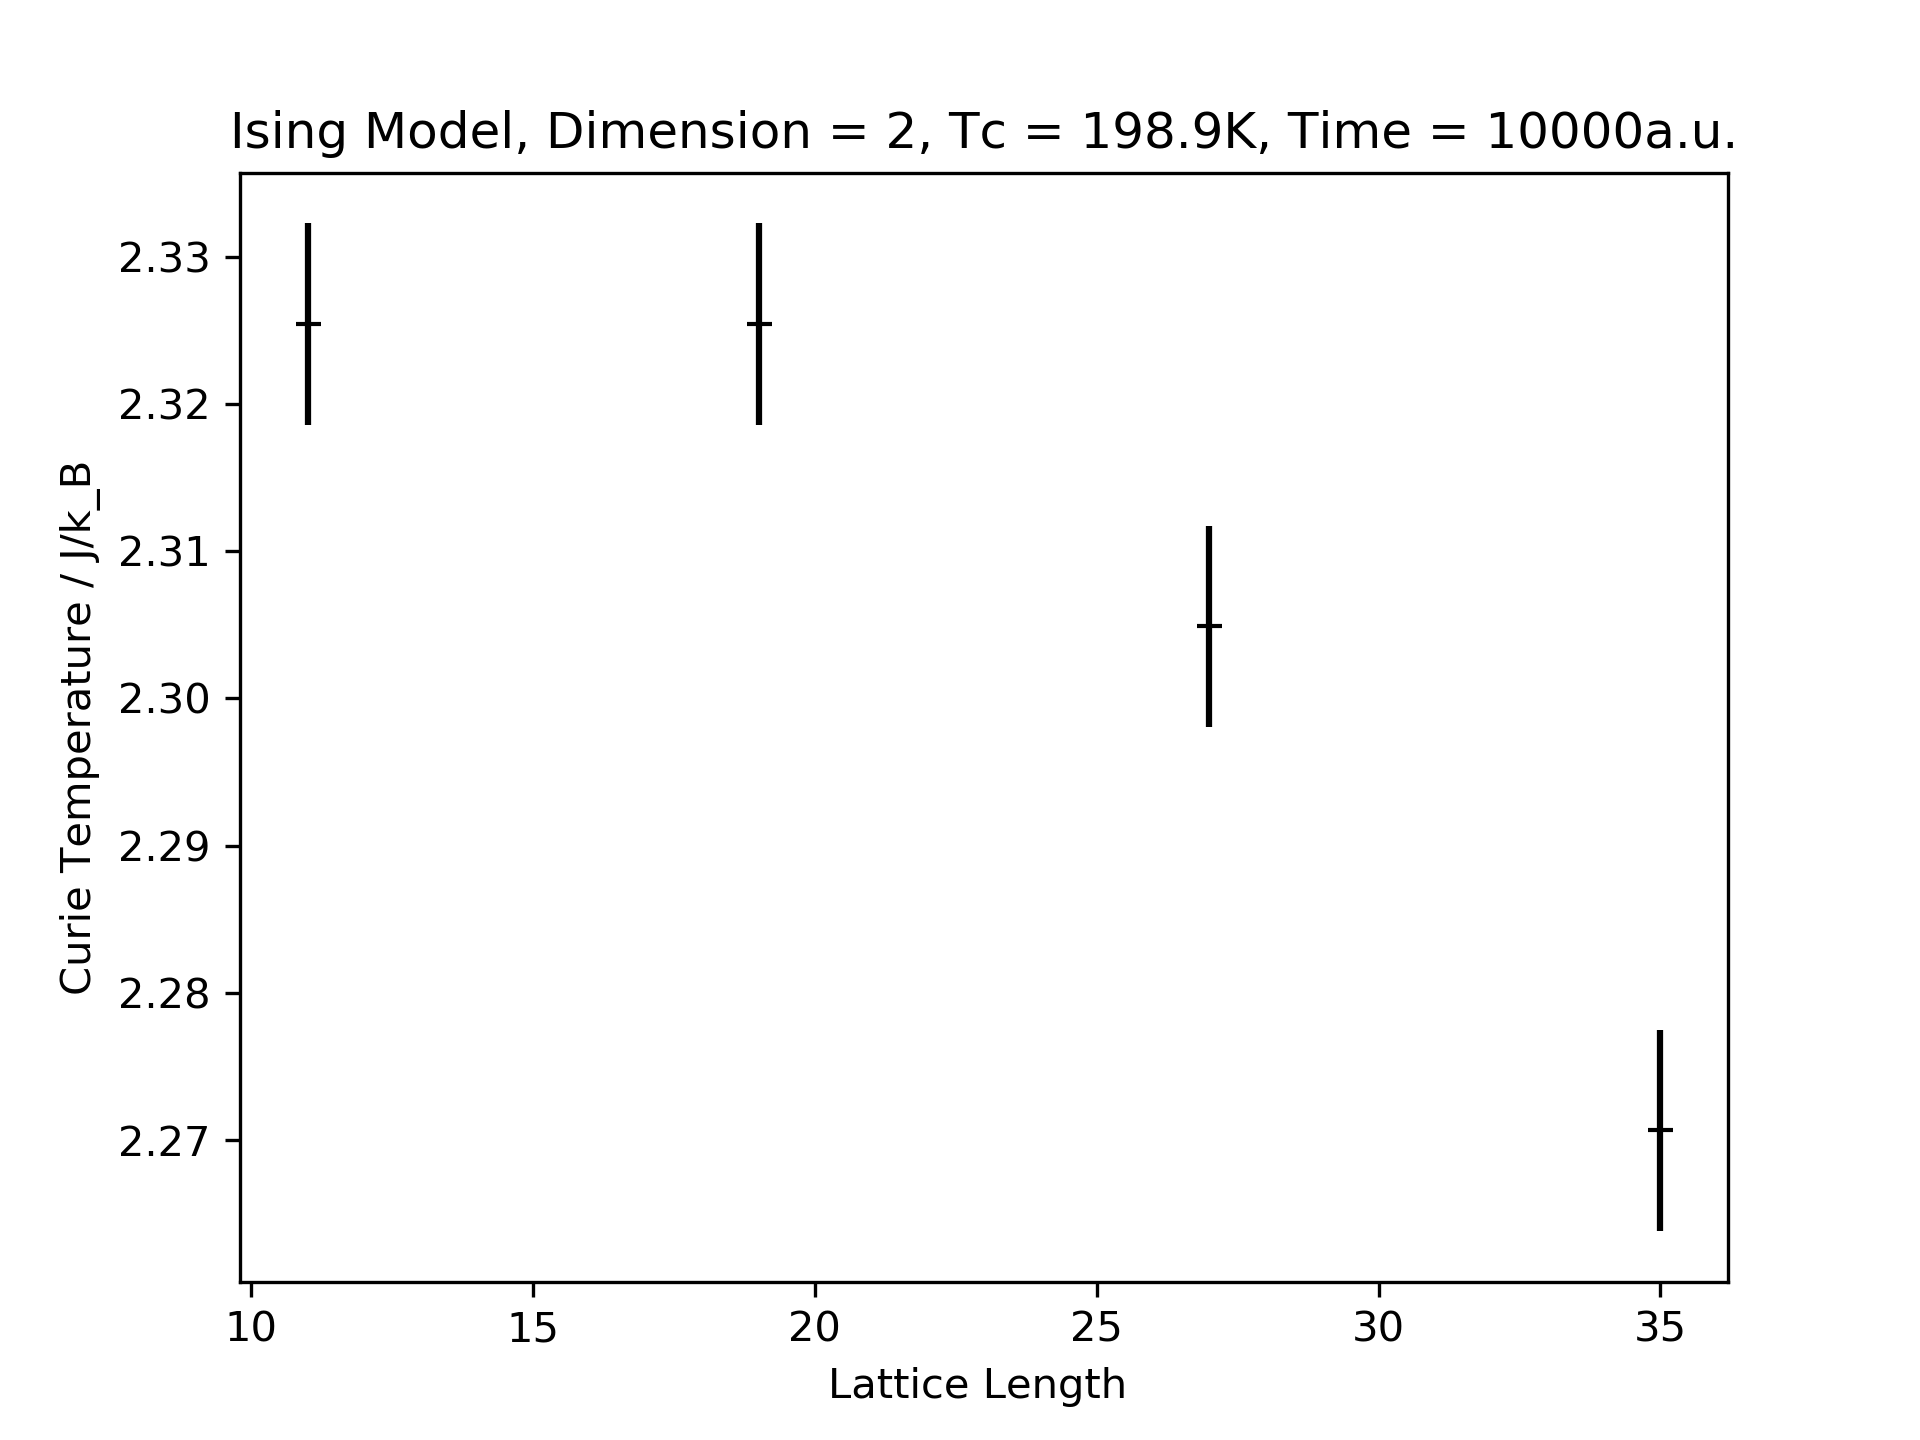
\includegraphics[width=0.7\textwidth]{../figures/curie_temp_vs_size2}
	% \ctikzfig{../figures/mag_mag_200_80_0.5}
	\caption{\label{fig:curie_temp_vs_size2} Curie temperature against system size.}
\end{figure}

Our upper estimate (according to the scaling relation \ref{eq:finite_size_scaling}) is $T_C = \SI{2.270(7)}{}$ \ref{fig:curie_temp_vs_size2}, with theoretical prediction $T_C = \SI{2.269}{}$ \ref{eq:curie_temp} lying just within 1 standard deviations. The data verified that Curie temperature decreases as systems size increases according to the finite-size scaling relation \ref{eq:finite_size_scaling}.

\begin{figure}[H] \centering
	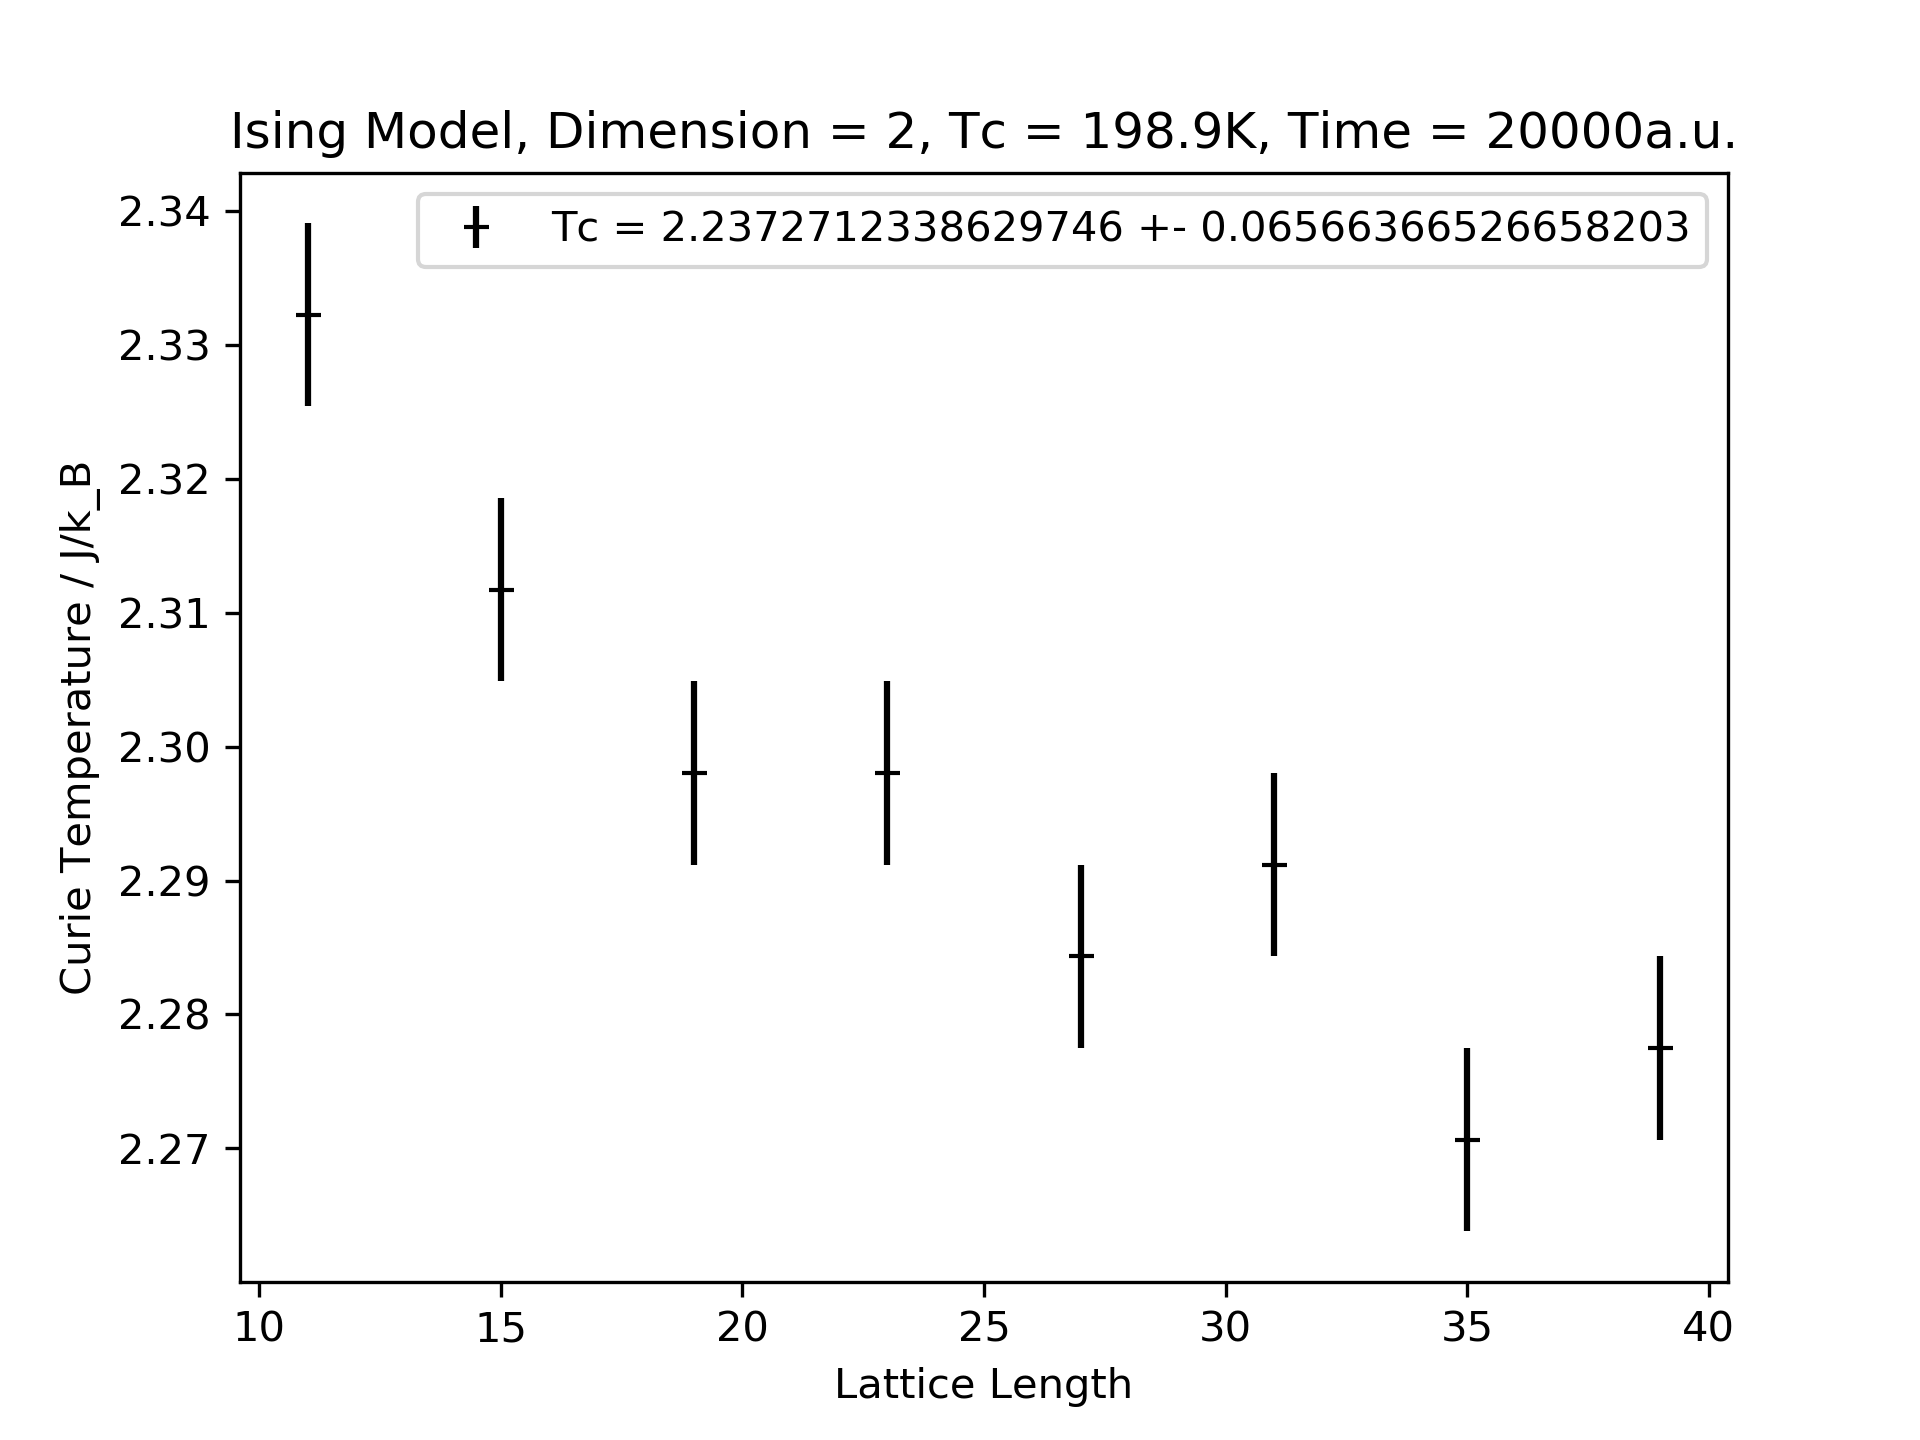
\includegraphics[width=0.7\textwidth]{../figures/finite_size}
	% \ctikzfig{../figures/mag_mag_200_80_0.5}
	\caption{\label{fig:finite_size} Finite size scaling of Curie temperature against system size.}
\end{figure}
By fitting \ref{eq:finite_size_scaling} using least square procedure (scipy.optimize.fit\_curve) and considering the error in Curie temperatures, we estimated $T_C(\infty) = \SI{2.24(7)}{}$ \ref{fig:finite_size}. Theoretical prediction lies within 1 standard deviation, justifying the correctness of the simulation.

A down shift in simulated Curie temperature is observed for both $T_C(specific\ heat) = \SI{196(6)}{}$ and $T_C(correlation\ time) = \SI{191}{\kelvin}$ as compared to theoretical prediction $T_C(theory) = \SI{198.9}{\kelvin}$. 

\section{\label{sec:hysteresis}Hysteresis Simulation}
Hysteresis effect appears when the system undergoes cyclic load (external field). The Dissipation energy per site for switching the Ising model is plotted against temperature.

\subsection{\label{sec:level2}Method}

\begin{algorithm}[H]
	\setstretch{1.35} 
	\caption{Ferromagnetic Hysteresis}
	\label{alg:hysteresis}
	\begin{algorithmic}
		\REQUIRE ~~\\
		All sites' spins initialized from a binary distribution;\\
		\label{code:hysteresis:initialize}
		\ENSURE ~~\\
		Evolve the system for a time $1.25 * T$, where T is the period of a sawtooth wave time varying external magnetic field;\\
		\label{code:hysteresis:}
	\end{algorithmic}
\end{algorithm}

Extra 0.25 cycle is simulated to remove initial state. Prolonged hysteresis loops can be produced using \ref{alg:hysteresis} with more periods. The external field's time dependence in a cycle is given below.

H(t)=
$\left\{
\begin{array}{cc}
	-H_0 \times t,& \for 0\leqslant t \leqslant T/4 \\
	-H_0 \times (T/2-t),& \for T/4\leqslant t \leqslant T/2 \\
	+H_0 \times (t-T/2),& \for T/2\leqslant t \leqslant 3T/4 \\
	+H_0 \times (T-t),& \for 3T/4\leqslant t \leqslant T
\end{array}
\right
.$

\begin{algorithm}[H]
	\setstretch{1.35} 
	\caption{Measuring Dissipation Energy}
	\label{alg:dissipation}
	\begin{algorithmic}
		\REQUIRE ~~\\
		System evolved for 0.25 + n cycles of length T;\\
		\label{code:hysteresis:initialize}
		\ENSURE ~~\\
		Excluding the initial 0.25 cycle;\\
		Set dissipation energy E = 0;\\
		Within each remaining cycle, Action(t)=
		$\left\{
		\begin{array}{cc}
		E+=-M(t) \times H_0 / (T/4),& \for 0\leqslant t \leqslant T/4 \\
		E+=-M(t) \times H_0 / (T/4),& \for T/4\leqslant t \leqslant T/2 \\
		E+=+M(t) \times H_0 / (T/4),& \for T/2\leqslant t \leqslant 3T/4 \\
		E+=+M(t) \times H_0 / (T/4),& \for 3T/4\leqslant t \leqslant T
		\end{array}
		\right
		.$\\
		Return $\frac{E}{n * N^2}$ where N is the lattice size.
		
		\label{code:hysteresis:}
	\end{algorithmic}
\end{algorithm}

\subsection{\label{sec:level2}Result}

\begin{figure}[H] \centering
	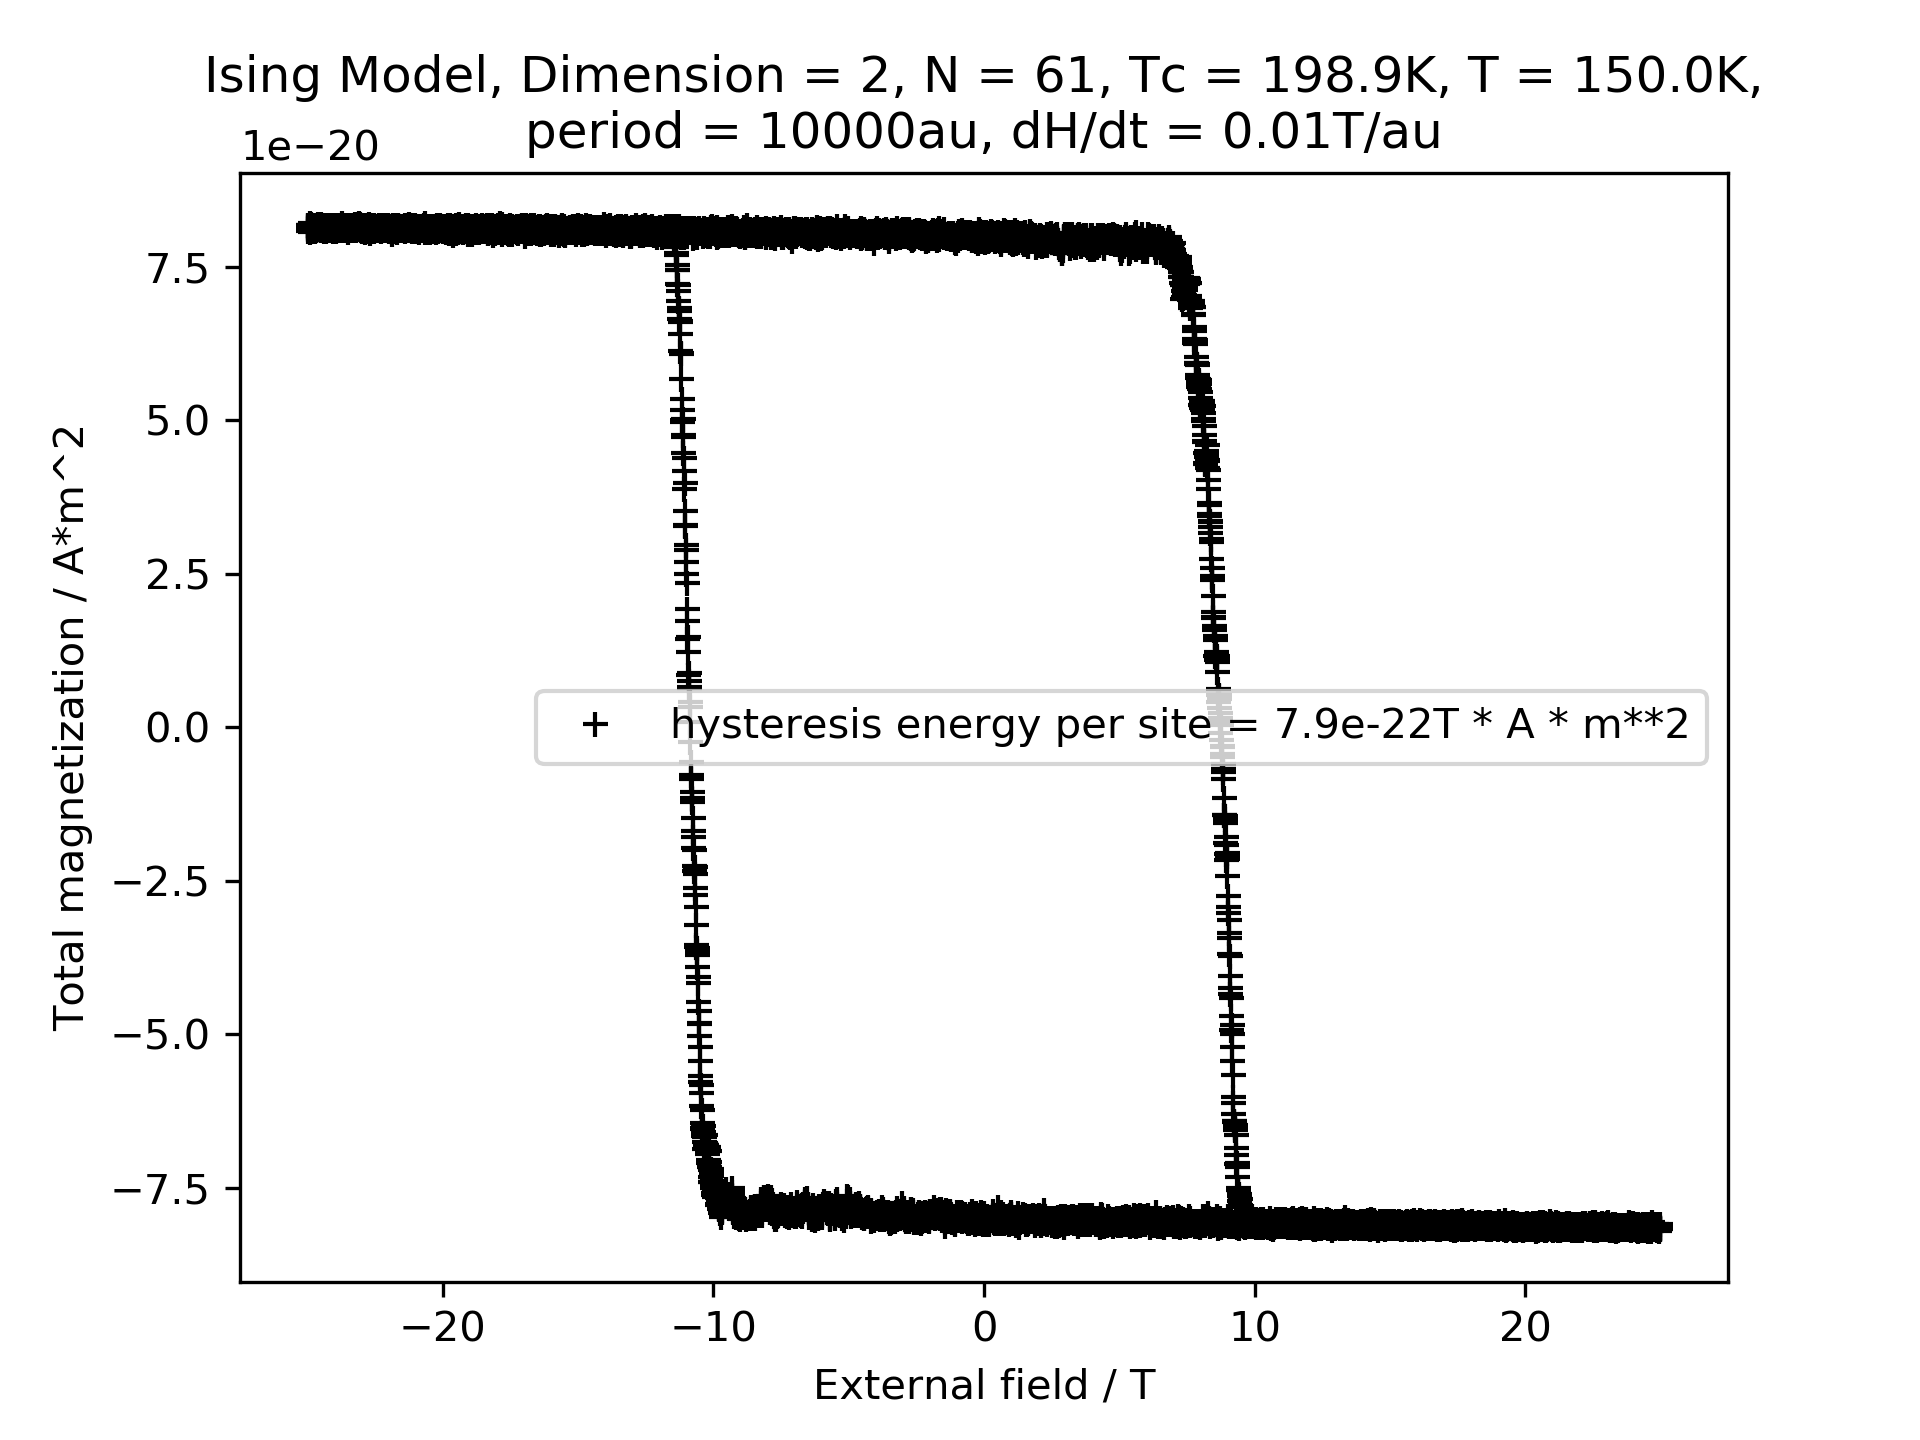
\includegraphics[width=0.7\textwidth]{../figures/hysteresis_scan}
	% \ctikzfig{../figures/mag_mag_200_80_0.5}
	\caption{\label{fig:hysteresis_scan} Finite size scaling of Curie temperature against system size.}
\end{figure}

At $150K$ our system exhibits hysteresis behaviour \ref{fig:hysteresis_scan}. 

\begin{figure}[H] \centering
	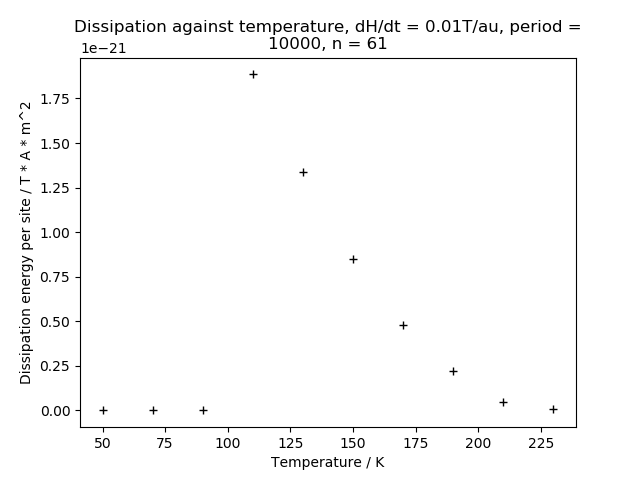
\includegraphics[width=0.7\textwidth]{../figures/hysteresis_dissipation}
	% \ctikzfig{../figures/mag_mag_200_80_0.5}
	\caption{\label{fig:hysteresis_dissipation} Dissipation energy per site against temperature.}
\end{figure}

In disordered phase, little dissipation is observed for the non-ferromagnetic system. In ordered phase, dissipation disappears below $110K$ \ref{fig:hysteresis_dissipation} as the external field fails to flip the system. Ferromagnetic strength decreases with temperature above $110K$.

\section{\label{sec:level1}Discussions}
The Checkerboard algorithm has enabled repeated calculation of large systems compared to the Metropolis algorithm. Near Curie point performance can still be improved using the Wolfson clustering. Temperature dependence of coercive field and saturation field can be studied in the future.


\section{\label{sec:level1}Summary}
Checkerboard algorithm \cite{BLOCK20101549} proves more efficient than the Metropolis algorithm as the system increase in size \ref{fig:metropolis_performance_no_rand}. Equilibrium time, correlation time, equilibrium magnetization, finite-size scaling and hysteresis behaviours corroborated theoretical analysis. 

This paper has 8286 words, with 4983 in the appendix, 59 in the summary and approximately 240 (10*24) in figure captions.

\section{\label{sec:level1}Appendix}

\begin{lstlisting}[language=Python]
# common computing and statistical packages
import numpy as np
import numpy.linalg as linalg
import scipy as sp
import scipy.stats
import statsmodels.tsa.stattools
import random
import time
import copy

# local convolution for local interaction energy
from scipy.ndimage import convolve, generate_binary_structure
from scipy.optimize import curve_fit

# error estimators
from astropy.stats import jackknife_stats
from astropy.stats import bootstrap

# Gaussian clustering
from itertools import cycle
from sklearn import mixture

import os  # writing to path
import sigfig  # rounding for data in plot title
from textwrap3 import wrap

import matplotlib as mpl
mpl.use('Agg')
from matplotlib import pyplot as plt

# -------------------------------------------------------------------------------

# SI Units ommited

# @jitclass(spec)
class Ising:
    # iron from https://www.southampton.ac.uk/~rpb/thesis/node18.html
    def __init__(self, name="none", N=100, H=0, T=273.15, D=2, J=1.21 * np.power(10.0, -21), randomFill=True, K=1.38064852 * np.power(10.0, -23), M=2.22 * np.power(10.0, (-23)), correlationTime=2, equilibriumTime=200, numberOfMeasurements=15):
        self.removeUnderflow = np.power(10, 0)
        self.j = J  # / self.removeUnderflow  # 'numerical' coupling constant
        self.h = H  # external field strength
        self.n = N  # lattice size
        self.m = M  # single spin magnetic moment
        self.k = K  # boltzman constant
        self.t = T  # / self.removeUnderflow # temperature in kelvins
        self.d = D  # system dimension
        self.tc = 2*J/(K*np.arcsinh(1))  # theoretical tc for 2d by onsanger
        self.timeStep = 0  # initialize timestep marker
        # figure sizes
        self.figureScale = 2
        self.figureDpi = 300 # matplotlib defaults to dpi=100
        # in inches
        self.figureHeight = 4.8
        self.figureWidth = 6.4
        # working
        self.kernel = generate_binary_structure(self.d, 1)
        self.ground = np.full(np.repeat(self.n, self.d), 0)
        # storage of system physical property time series: time stamp, total magnetization, total energy,
        self.systemDataTimeSeries = [[], [], []]
        # storage of blocksize, measured magnetization, variance of measured magnetization, variance in that variance
        self.correlationTimeEstimates = [[], [], []]
        self.binderCumulant = None
        # normalized magnetization auto-covariance
        self.normalizedMagnetizationAutocovariance = None
        # Time needed to reach steady state from initial state, initially set to zero
        # will be updated if systems takes time t to move into equilibrium

        # mean magnetization and its error from a single measurement, returned as a 2 element list
        self.meanMagnetizationWithError = []

        self.equilibriumTime = equilibriumTime
        self.numberOfMeasurements = numberOfMeasurements
        # correlation time initially set to 2
        # can be precomputed then provided
        # Warning: THIS IS A REAL
        self.correlationTime = correlationTime
        # this cannot be provided
        self.specificHeatCapacityPerSite = None
        # plotting colors
        self.colors_ = cycle(mpl.colors.TABLEAU_COLORS.keys())

        # define the system with or without initial values
        spins = [1, -1]
        if randomFill:
            self.system = np.random.choice(spins, tuple(np.repeat(self.n, self.d)))
        else:
            # dangerously, for future importing of existing system
            # currently randomly chooses all up or all down
            self.system = np.full(tuple(np.repeat(self.n, self.d)), np.choose(1, [1, -1]))
        self.system = np.asarray(self.system)
        choices = list(range(self.n**self.d))

        # warning: optimization only works in odd sized dimensions!!!
        zerothSites = choices[0::4]
        firstSites = choices[1::4]
        secondSites = choices[2::4]
        thirdSites = choices[3::4]
        # notice we still have the difficulty of flipping large domains with smooth boundaries at especially low temperatures


        # dimension index
        self.dimensions = range(self.d)

        # zerothLattice
        self.zerothLattice = np.full(tuple(np.repeat(self.n, self.d)), False)
        for choice in zerothSites:
            self.zerothLattice[tuple([int(np.floor(choice % self.n**(x+1) / self.n**x)) for x in self.dimensions])] = True

        # firstLattice
        self.firstLattice = np.full(tuple(np.repeat(self.n, self.d)), False)
        for choice in firstSites:
            self.firstLattice[tuple([int(np.floor(choice % self.n**(x+1) / self.n**x)) for x in self.dimensions])] = True

        # secondLattice
        self.secondLattice = np.full(tuple(np.repeat(self.n, self.d)), False)
        for choice in secondSites:
            self.secondLattice[tuple([int(np.floor(choice % self.n**(x+1) / self.n**x)) for x in self.dimensions])] = True

        # thirdLattice
        self.thirdLattice = np.full(tuple(np.repeat(self.n, self.d)), False)
        for choice in thirdSites:
            self.thirdLattice[tuple([int(np.floor(choice % self.n**(x+1) / self.n**x)) for x in self.dimensions])] = True

        # in each step randomly update all sublattices
        self.sublattices = np.array([self.zerothLattice, self.firstLattice, self.secondLattice, self.thirdLattice])

        # self.evenLattice = np.invert(copy.deepcopy(self.oddLattice))
        # iniitalize initial energies using initial state
        self.updateEnergies()

        # save initial system data at time stamp=0
        self.systemDataTimeSeries[0].append(self.timeStep)
        self.systemDataTimeSeries[1].append(self.totalMagnetization())
        # care: coordination number normalization when accounting for total energy
        self.systemDataTimeSeries[2].append(np.sum(self.interactionEnergies) / 2)

        self.stationaryMagnetization = None

    def totalMagnetization(self):
        return self.m * np.sum(self.system)

    # Warning: estimate the equilibrium time before calculating binderCumulent
    def estimateBinderCumulant(self):
        data = copy.deepcopy(self.systemDataTimeSeries)
        # crop transients
        if not self.equilibriumTime == 0:
            data[0] = data[0][slice(int(self.equilibriumTime * 2), self.timeStep)]
            data[1] = data[1][slice(int(self.equilibriumTime * 2), self.timeStep)]
            data[2] = data[2][slice(int(self.equilibriumTime * 2), self.timeStep)]
        meanToTheFourth = np.mean(np.power(data[1], 4.0))
        meanToTheSecond = np.mean(np.power(data[1], 2.0))
        self.binderCumulant = 1 - meanToTheFourth / (3 * meanToTheSecond ** 2)

    def localEnergy(self, coords):  # periodic bc
        # coords a list contain d integer indices to specify the ising lattice in d dimensional space
        sumOfNeighbours = 0
        for i in range(len(coords)):  # traverse in f/b directions
            coordsCopy = copy.deepcopy(coords)  # deep copy by default
            coordsCopy[i] = (coords[i] + 1) % self.n
            sumOfNeighbours += self.system[tuple([[x] for x in coordsCopy])][0]
            coordsCopy[i] = (coordsCopy[i] - 2) % self.n
            sumOfNeighbours += self.system[tuple([[x] for x in coordsCopy])][0]

        coords = tuple([[x] for x in coords])
        return (- self.j * (self.system[coords]) * sumOfNeighbours +
                self.m * self.h * self.system[coords])[0]
        # coupling energy + external field interaction

    # function for parallel update of interaction energies
    def updateEnergies(self):
        self.interactionEnergies = \
                (-self.j) * (convolve(self.system, self.kernel, mode='wrap') - self.system) * self.system + \
                self.m * self.h * self.system

    # currently deprecated
    def flip(self, coords):
        energy = self.localEnergy(coords)
        # print(energy)
        coords = tuple([[x] for x in coords])
        if energy >= 0:  # flip
            self.system[coords] *= -1
        else:
            boltzmanFactor = np.exp(2*energy/(self.k * self.t))
            # p = random.uniform(0, 1)
            if random.randint(0, 1) < boltzmanFactor: self.system[coords] = -self.system[coords]

    def visualizeMagnetization(self, path="noPath.png", hyperplane=None):
        # plots the total magnetization with time
        plt.close()
        fig = plt.figure(figsize=(self.figureWidth * self.figureScale, self.figureHeight * self.figureScale), dpi=self.figureDpi)
        # fig = plt.figure()
        plt.plot(self.systemDataTimeSeries[0], self.systemDataTimeSeries[1], "+k")
        plt.axvline(x=self.equilibriumTime)
        plt.title("\n".join(wrap("Ising Model, Dimension = "+str(self.d)+", N = "+str(self.n)+", Tc = "+str(sigfig.round(float(self.tc), sigfigs=4))+"K, T = "+str(sigfig.round(float(self.t), sigfigs=4)) + "K, Time = "+str(self.timeStep)+"au", 60)))
        plt.xlabel("Time steps / a.u.")
        plt.ylabel("Total magnetization / Am^2")
        return fig

    def visualizeTotalEnergy(self, path="noPath.png", hyperplane=None):
        # plots the total magnetization with time
        plt.close()
        # fig = plt.figure()
        fig = plt.figure(figsize=(self.figureWidth * self.figureScale, self.figureHeight * self.figureScale), dpi=self.figureDpi)
        plt.plot(self.systemDataTimeSeries[0], self.systemDataTimeSeries[2], "+k")
        plt.axvline(x=self.equilibriumTime)
        plt.title("\n".join(wrap("Ising Model, Dimension = "+str(self.d)+", N = "+str(self.n)+", Tc = "+str(sigfig.round(float(self.tc), sigfigs=4))+"K, T = "+str(sigfig.round(float(self.t), sigfigs=4)) + "K, Time = "+str(self.timeStep)+"au", 60)))
        plt.xlabel("Time steps / a.u.")
        plt.ylabel("Total energy / J")
        return fig

    def meanStationaryMagnetization(self, path="noPath.png", hyperplane=None):
        # calculate mean stationary magnetization and its variance
        # return a two element list

        # remove the transient data
        if not self.equilibriumTime == 0:
            steadyStateDataTimeSeries = copy.deepcopy(self.systemDataTimeSeries[1][slice(int(self.equilibriumTime * 2), self.timeStep)])
        else:
            steadyStateDataTimeSeries = copy.deepcopy(self.systemDataTimeSeries[1])
        blockSize = int(self.correlationTime) + 1
        numberOfMeasurements = self.numberOfMeasurements

        # measure in blocks of size the correlation length
        averages = np.array([])
        for i in range(numberOfMeasurements):
            if (i + 1) * blockSize < len(steadyStateDataTimeSeries): # prevent running off indices
                averages = np.append(averages, [np.mean(steadyStateDataTimeSeries[slice(i * blockSize, (i + 1) * blockSize)])])
            else:
                break

        self.stationaryMagnetization = [np.mean(averages), np.sqrt(np.var(averages) / (self.numberOfMeasurements - 1))]
        return self.stationaryMagnetization

    def visualizeMagnetizationAutocovariance(self, path="noPath.png", hyperplane=None):
        plt.close()
        fig = plt.figure(figsize=(self.figureWidth * self.figureScale, self.figureHeight * self.figureScale), dpi=self.figureDpi)
        data = copy.deepcopy(self.systemDataTimeSeries)
        # crop transients
        if not self.equilibriumTime == 0:
            data[0] = data[0][slice(int(self.equilibriumTime * 2), self.timeStep)]
            data[1] = data[1][slice(int(self.equilibriumTime * 2), self.timeStep)]
            data[2] = data[2][slice(int(self.equilibriumTime * 2), self.timeStep)]

        # returns an auto-covariance plot
        magnetizationAutocovariance = statsmodels.tsa.stattools.acovf(data[1], demean=True, fft=True)
        # with non-equilibrium cropped
        normalizedMagnetizationAutocovariance = magnetizationAutocovariance/magnetizationAutocovariance[0]
        # save current autocovariance
        self.normalizedMagnetizationAutocovariance = normalizedMagnetizationAutocovariance
        # fig = plt.figure()
        plt.plot(data[0], normalizedMagnetizationAutocovariance, "+k")
        plt.axvline(x=self.equilibriumTime)
        plt.title("\n".join(wrap("Ising Model, Dimension = "+str(self.d)+", N = "+str(self.n)+", Tc = "+str(sigfig.round(float(self.tc), sigfigs=4))+"K, T = "+str(sigfig.round(float(self.t), sigfigs=4)) + "K, Time = "+str(self.timeStep)+"au", 60)))
        plt.xlabel("Time steps / a.u.")
        plt.ylabel("Auto-covariance of magnetization")
        return fig

    # warning, only estimate the correlation time after computing the auto-covariance time series
    def estimateCorrelationTime(self):
        cropLength = 0
        cropFinished = False
        # case where correlation time is not estimated is not handled here
        for i in range(self.timeStep - int(self.equilibriumTime * 2)):
            if cropFinished:
                break
            if self.normalizedMagnetizationAutocovariance[i] <= np.exp(-2.0):
                cropLength = i
                cropFinished = True

        # this is a more sophisticated method by fitting the autocovariance curve
        """
        croppedAutocovariance = copy.deepcopy(self.normalizedMagnetizationAutocovariance[:cropLength])
        time = np.arange(cropLength)

        # print(croppedAutocovariance)
        logCroppedAutocovariance = np.log(croppedAutocovariance)
        # logTime = np.log(time)
        b, m = np.polyfit(time, logCroppedAutocovariance, 1)
        self.correlationTime = np.absolute(1 / m)
        """
        self.correlationTime = cropLength

        # successfully estimated correlation time
        return True

    def estimateSpecificHeatCapacityPerSite(self):
        data = copy.deepcopy(self.systemDataTimeSeries)
        # crop transients
        if not self.equilibriumTime == 0:
            data[0] = data[0][slice(int(self.equilibriumTime * 2), self.timeStep)]
            data[1] = data[1][slice(int(self.equilibriumTime * 2), self.timeStep)]
            data[2] = data[2][slice(int(self.equilibriumTime * 2), self.timeStep)]
        energyTimeSeriesPerSite = data[2] / np.power(self.n, self.d)
        # fluctuation dissipation theorem
        specificHeatCapacityPerSite = np.sqrt((np.var(energyTimeSeriesPerSite))/(self.k * self.t**2))
        self.specificHeatCapacityPerSite = specificHeatCapacityPerSite
        return True

    # data cleaning function that demean and normalize data using its absolute magnitude
    def demeanNormalize(self, ndarray):
        ndarray = copy.deepcopy(ndarray)
        ndarray = ndarray / np.mean(np.absolute(ndarray))
        ndarray = ndarray - np.mean(ndarray)
        return ndarray

    # helper cluster data plotter from scikit-learn, note plots at 1, 2, n sub graph for comparison with the original
    def plotClustersEstimateEquilibriumTime(self, X, model, subplot):
        Y_ = model.predict(X)
        covariances = model.covariances_
        means = model.means_
        for i, (mean, covar, color) in enumerate(zip(
            means, covariances, self.colors_)):
        # for i, (mean, covar) in enumerate(zip(
        #     means, covariances)):
            v, w = linalg.eigh(covar)
            v = 2. * np.sqrt(2.) * np.sqrt(v)
            u = w[0] / linalg.norm(w[0])
            # as the DP will not use every component it has access to
            # unless it needs it, we shouldn't plot the redundant
            # components.
            if not np.any(Y_ == i):
                continue
            subplot.scatter(X[Y_ == i, 0], X[Y_ == i, 1], .8, color=color)

            # Plot an ellipse to show the Gaussian component
            angle = np.arctan(u[1] / u[0])
            angle = 180. * angle / np.pi  # convert to degrees
            ell = mpl.patches.Ellipse(mean, v[0], v[1], 180. + angle, color=color)
            ell.set_clip_box(subplot.bbox)
            ell.set_alpha(0.5)
            subplot.add_artist(ell)

        # identify number of steps to equilibrium, if any steps needed at all
        modelLabels = Y_
        labels, counts = np.unique(modelLabels[modelLabels >= 0], return_counts=True)
        if np.absolute(counts[0] - counts[1]) / self.timeStep < 0.5:
            self.equilibriumTime = 0
            print("Either already in equilibrium state or system has not reached equilibrium. \nEquilibrium time defaults to 0.")
        else:
            self.equilibriumTime = np.amin(counts)
            print("Time to equilibrium: " + str(self.equilibriumTime))

    def visualizeMagnetizationPhaseSpace(self, path="noPath.png", hyperplane=None):
        # plots the total magnetization with its time
        plt.close()
        fig = plt.figure(figsize=(self.figureWidth * self.figureScale * 2, self.figureHeight * self.figureScale), dpi=self.figureDpi)
        # import and reshape data
        # scikit-learn only takes columns of attributes
        magnetization = self.demeanNormalize(self.systemDataTimeSeries[1])
        magnetization = np.reshape(magnetization, (magnetization.size, 1))
        magnetizationGradient = self.demeanNormalize(np.gradient(self.systemDataTimeSeries[1]))
        magnetizationGradient = np.reshape(magnetizationGradient, (magnetizationGradient.size, 1))

        # original data
        ax = fig.add_subplot(1, 2, 1)
        ax.plot(magnetization, magnetizationGradient, "+k")
        plt.title("\n".join(wrap("Ising Model, Dimension = "+str(self.d)+", N = "+str(self.n)+", Tc = "+str(sigfig.round(float(self.tc), sigfigs=4))+"K, T = "+str(sigfig.round(float(self.t), sigfigs=4)) + "K, Time = "+str(self.timeStep)+"au", 60)))
        plt.xlabel("demeaned and magnitude normalized Magnetization / a.u.")
        plt.ylabel("d(demeaned and magnitude normalized Magnetization)/dt / a.u.")

        # clustering using scikit.learn
        X = np.hstack((magnetization, magnetizationGradient))
        # model = Birch(threshold=0.5, n_clusters=2)
        # model = KMeans(n_clusters=2)
        model = mixture.GaussianMixture(n_components=2, covariance_type='full')
        model.fit(X)
        ax = fig.add_subplot(1, 2, 2)
        self.plotClustersEstimateEquilibriumTime(X, model, ax)
        plt.title("\n".join(wrap("Ising Model, Dimension = "+str(self.d)+", N = "+str(self.n)+", Tc = "+str(sigfig.round(float(self.tc), sigfigs=4))+"K, T = "+str(sigfig.round(float(self.t), sigfigs=4)) + "K, Time = "+str(self.timeStep)+"au", 60)))
        plt.xlabel("demeaned and magnitude normalized Magnetization / a.u.")
        plt.ylabel("d(demeaned and magnitude normalized Magnetization)/dt / a.u.")
        return fig

    def visualizeTwoDGrid(self, path="noPath.png", hyperplane=None):
        # safety measure: close all plots
        plt.close()
        # hyperplane should be an integer indexing list
        cmap = mpl.colors.ListedColormap(['white', 'black'])
        bounds = [-1, 0, 1]
        norm = mpl.colors.BoundaryNorm(bounds, cmap.N)
        # data reshape
        data = copy.deepcopy(self.system[hyperplane])
        if data.shape == tuple([self.n, self.n]):
            pass
        else:
            data = data[:, :, 0]
        # plot
        fig, axes = plt.subplots()
        fig = plt.figure(figsize=(self.figureWidth * self.figureScale, self.figureHeight * self.figureScale))
        axes = fig.add_subplot(111)
        img = axes.imshow(data, interpolation='nearest', cmap=cmap, norm=norm, animated=True)

        plt.colorbar(img, cmap=cmap, norm=norm, boundaries=bounds, ticks=[-1, 0, 1])
        plt.title("\n".join(wrap("Ising Model, Dimension = "+str(self.d)+", N = "+str(self.n)+", Tc = "+str(sigfig.round(float(self.tc), sigfigs=4))+"K, T = "+str(sigfig.round(float(self.t), sigfigs=4)) + "K, Time = "+str(self.timeStep)+"au", 60)))
        return fig

    # warning: do not run on its own
    # this is a helper function for stepForward()
    def updateSublattice(self, sublattice):
        boltzmanFactor = np.exp(2 * self.interactionEnergies / (self.k * self.t))
        evenDist = np.random.uniform(0, 1, size=np.repeat(self.n, self.d))
        temp1 = np.greater(self.interactionEnergies, self.ground)
        temp2 = np.greater(boltzmanFactor, evenDist)
        criteria = np.logical_and(sublattice, np.logical_or(temp1, temp2))
        self.system = np.where(criteria, -self.system, self.system)
        self.updateEnergies()

    def stepForward(self):
        # stepping through the lattice and update randomly
        # improved method: divide into two sub-lattices and vectorize for each sub lattice to allow batch processing
        # note that a site cannot be updated twice within a single step, and two neighbouring sites should not be updated simultaneously
        self.timeStep = self.timeStep + 1

        np.random.shuffle(self.sublattices)
        for sublattice in self.sublattices:
            self.updateSublattice(sublattice)

        # record system data
        self.systemDataTimeSeries[0].append(self.timeStep)
        self.systemDataTimeSeries[1].append(self.totalMagnetization())
        # care: coordination number normalization when accounting for total energy to avoid double counting
        self.systemDataTimeSeries[2].append(np.sum(self.interactionEnergies) / 2)


# ----------------------------------------------------------------------------------------
# calculate the time evolution of a 2 D ising model system given the predefined parameters


# working now: investigate the hysteresis effect in a 2 d system
# the hysteresis by cycling h
# measure the remnant field
# measure the external field needed for total negating of the field
# measure the hysteresis loop energy, notice need to add impurities if you want a considerable amount of area enclosed

# measurement class to allow taking measurements across multiple systems
# @jitclass(spec)
class InquireIsing:
    def __init__(self, name="none", N=100, H=0, T=273.15, D=2, J=1.21 * np.power(10.0, -21), randomFill=True, K=1.38064852 * np.power(10.0, -23), M=2.22 * np.power(10.0, (-23)), correlationTime=20, equilibriumTime=0, steps=1500, numberOfMeasurements=15, dataPoints=10, lowerTemperature=20, deltaTemperature = 20):
        self.removeUnderflow = np.power(10, 0)
        self.j = J  # / self.removeUnderflow  # 'numerical' coupling constant
        self.h = H  # external field strength
        self.n = N  # lattice size
        self.m = M  # single spin magnetic moment
        self.k = K  # boltzman constant
        self.t = T  # / self.removeUnderflow # temperature in kelvins
        self.d = D  # system dimension
        self.tc = 2*J/(K*np.arcsinh(1))  # theoretical tc for 2d by onsanger
        self.randomFill = randomFill
        self.steps = steps
        self.numberOfMeasurements = numberOfMeasurements
        self.dataPoints = dataPoints
        self.lowerTemperature = lowerTemperature
        self.deltaTemperature = deltaTemperature
        # figure sizes
        self.figureScale = 1
        self.figureDpi = 300 # matplotlib defaults to dpi=100
        # in inches
        self.figureHeight = 4.8
        self.figureWidth = 6.4
        # Time needed to reach steady state from initial state, initially set to zero
        # will be updated if systems takes time t to move into equilibrium
        self.equilibriumTime = equilibriumTime
        self.name = name
        # correlation time initially set to 2
        # can be inputed if precomputed
        self.correlationTime = correlationTime
        # plotting colors
        # self.colors_ = cycle(mpl.colors.TABLEAU_COLORS.keys())

        # data
        # size of block, mean variance in mean steady state magnetization, variance in the variance
        # self.blockSizeAndVarianceInMeanMagnetization = [[], [], []]
        self.meanStationaryMagnetizationAgainstTemperature = None
        self.equilibriumTimeAgainstTemperature = None
        self.correlationTimeAgainstTemperature = None
        self.binderCumulantAgainstTemperature = None
        self.specificHeatCapacityPerSiteAgainstTemperature = None

    def visualizeBinderCumulant(self):
        # plots the average magnetization vs number of blocks used for measurement
        # when the variance starts to grow wildly, we choose the largest block size with non-diverging error as our correlation length (or time)
        plt.close()
        lowerTemperature = self.lowerTemperature
        deltaTemperature = self.deltaTemperature
        numberOfMeasurements = self.numberOfMeasurements
        attempts = self.dataPoints
        # temperature and equilibriumTime and error
        data = [[], [], []]
        for a in range(attempts):
            temperature = lowerTemperature + a * deltaTemperature
            data[0].append(temperature)
            binderCumulants = []
            for j in range(numberOfMeasurements):
                tempSys = Ising(name=self.name, N=self.n, H=self.h, T=temperature, D=self.d, J=self.j, randomFill=self.randomFill, K=self.k, M=self.m, equilibriumTime=self.equilibriumTime)
                for i in range(self.steps):
                    tempSys.stepForward()
                # estimate equilibrium time needed
                tempSys.visualizeMagnetizationPhaseSpace()
                tempSys.estimateBinderCumulant()
                binderCumulants.append(tempSys.binderCumulant)
                # [meanMagnetization, errorMagnetization] = tempSys.meanStationaryMagnetization()
                # errors.append(errorMagnetization)
            data[1].append(np.mean(binderCumulants))
            
            # three ways to estimate errors
            _input = np.array(binderCumulants)
            _statistics = np.mean
            
            sem = scipy.stats.sem(_input) # only works for mean
            jackknife_estimate, bias, stderr, conf_interval = jackknife_stats(np.array(_input), _statistics, 0.682)
            bootstrap_estimate = bootstrap(_input, bootfunc=_statistics)
            
            data[2].append(jackknife_estimate)
            
        # update stored data
        self.binderCumulantAgainstTemperature = data
        # fig = plt.figure()
        fig = plt.figure(figsize=(self.figureWidth * self.figureScale, self.figureHeight * self.figureScale), dpi=self.figureDpi)
        # print(self.blockSizeAndVarianceInMeanMagnetization)
        plt.errorbar(self.binderCumulantAgainstTemperature[0], self.binderCumulantAgainstTemperature[1], yerr=self.binderCumulantAgainstTemperature[2], fmt="+k")
        # plt.axvline(x=self.equilibriumTime)
        plt.title("\n".join(wrap("Ising Model, Dimension = "+str(tempSys.d)+", N = "+str(tempSys.n)+", Tc = "+str(sigfig.round(float(tempSys.tc), sigfigs=4))+"K, Time = "+str(tempSys.timeStep)+"a.u.", 60)))
        plt.xlabel("Temperature / K")
        plt.ylabel("Binder Cumulant / 1")
        return fig



    def visualizeEquilibriumTime(self):
        # plots the average magnetization vs number of blocks used for measurement
        # when the variance starts to grow wildly, we choose the largest block size with non-diverging error as our correlation length (or time)
        plt.close()
        lowerTemperature = self.lowerTemperature
        deltaTemperature = self.deltaTemperature
        numberOfMeasurements = self.numberOfMeasurements
        attempts = self.dataPoints
        # temperature and equilibriumTime and error
        data = [[], [], []]
        for a in range(attempts):
            temperature = lowerTemperature + a * deltaTemperature
            data[0].append(temperature)
            # self.blockSizeAndVarianceInMeanMagnetization[0].append(blockSize)
            equilibriumTimes = []
            for j in range(numberOfMeasurements):
                tempSys = Ising(name=self.name, N=self.n, H=self.h, T=temperature, D=self.d, J=self.j, randomFill=self.randomFill, K=self.k, M=self.m, equilibriumTime=self.equilibriumTime)
                for i in range(self.steps):
                    tempSys.stepForward()
                # estimate equilibrium time needed
                tempSys.visualizeMagnetizationPhaseSpace()
                equilibriumTimes.append(tempSys.equilibriumTime)
                # [meanMagnetization, errorMagnetization] = tempSys.meanStationaryMagnetization()
                # errors.append(errorMagnetization)
            data[1].append(np.mean(equilibriumTimes))
            data[2].append(np.sqrt(np.var(equilibriumTimes)))
        # update stored data
        self.equilibriumTimeAgainstTemperature = data
        # fig = plt.figure()
        fig = plt.figure(figsize=(self.figureWidth * self.figureScale, self.figureHeight * self.figureScale), dpi=self.figureDpi)
        # print(self.blockSizeAndVarianceInMeanMagnetization)
        plt.errorbar(self.equilibriumTimeAgainstTemperature[0], self.equilibriumTimeAgainstTemperature[1], yerr=self.equilibriumTimeAgainstTemperature[2], fmt="+k")
        # plt.axvline(x=self.equilibriumTime)
        plt.title("\n".join(wrap("Ising Model, Dimension = "+str(tempSys.d)+", N = "+str(tempSys.n)+", Tc = "+str(sigfig.round(float(tempSys.tc), sigfigs=4))+"K, Time = "+str(tempSys.timeStep)+"a.u.", 60)))
        plt.xlabel("Temperature / K")
        plt.ylabel("Equilibrium Time / a.u.")
        return fig

    def visualizeStationaryMagnetization(self):
        # plots the average magnetization vs number of blocks used for measurement
        # when the variance starts to grow wildly, we choose the largest block size with non-diverging error as our correlation length (or time)
        plt.close()
        lowerTemperature = self.lowerTemperature
        deltaTemperature = self.deltaTemperature
        numberOfMeasurements = self.numberOfMeasurements
        dataPoints = self.dataPoints
        # temperature and mean magnetization and error
        data = [[], [], []]
        for a in range(dataPoints):
            temperature = lowerTemperature + a * deltaTemperature

            # compute the correlation time under current temp
            # !!! to be finished !!! 

            data[0].append(temperature)
            # self.blockSizeAndVarianceInMeanMagnetization[0].append(blockSize)
            tempSys = Ising(name=self.name, N=self.n, H=self.h, T=temperature, D=self.d, J=self.j, randomFill=self.randomFill, K=self.k, M=self.m, equilibriumTime=self.equilibriumTime, correlationTime=20, numberOfMeasurements=self.numberOfMeasurements)
            for step in range(self.steps):
                tempSys.stepForward()

            # necessary facilitating computations
            tempSys.visualizeMagnetizationPhaseSpace()
            tempSys.visualizeMagnetizationAutocovariance()
            tempSys.estimateCorrelationTime()
            print(tempSys.correlationTime)

            [meanMag, error] = tempSys.meanStationaryMagnetization()
            data[1].append(meanMag)
            data[2].append(error)
        # update stored data
        self.meanStationaryMagnetizationAgainstTemperature = data
        fig = plt.figure(figsize=(self.figureWidth * self.figureScale, self.figureHeight * self.figureScale), dpi=self.figureDpi)
        plt.errorbar(self.meanStationaryMagnetizationAgainstTemperature[0], self.meanStationaryMagnetizationAgainstTemperature[1], yerr=self.meanStationaryMagnetizationAgainstTemperature[2], fmt="+k")
        plt.title("\n".join(wrap("Ising Model, Dimension = "+str(self.d)+", N = "+str(self.n)+", Tc = "+str(sigfig.round(float(self.tc), sigfigs=4))+"K, Time = "+str(self.steps)+"a.u.", 60)))
        plt.xlabel("Temperature / K")
        plt.ylabel("Stationary Magnetization / Am^2")
        return fig

    # helper function returning correlation time for a specific temperature, keeping all other parameters as inputs
    # used in function visualizeCorrelationTime
    def correlationTimeByTemperature(self, T=200):
        correlationTimes = []
        j = 0
        while j < self.numberOfMeasurements:
            # use specified temperature
            tempSys = Ising(name=self.name, N=self.n, H=self.h, T=T, D=self.d, J=self.j, randomFill=self.randomFill, K=self.k, M=self.m, equilibriumTime=self.equilibriumTime, numberOfMeasurements=self.numberOfMeasurements)
            for step in range(self.steps):
                tempSys.stepForward()
            # estimate equilibrium time
            tempSys.visualizeMagnetizationPhaseSpace()
            # compute auto correlation time series
            tempSys.visualizeMagnetizationAutocovariance()
            # estimate correlation time
            tempSys.estimateCorrelationTime()
            j = j + 1
            correlationTimes.append(tempSys.correlationTime)
        return [np.mean(correlationTimes), np.sqrt(np.var(correlationTimes))]

    def visualizeCorrelationTime(self, n=31, delta=10, size=3):
        # plots the average magnetization vs number of blocks used for measurement
        # when the variance starts to grow wildly, we choose the largest block size with non-diverging error as our correlation length (or time)
        plt.close()
        lowerTemperature = self.lowerTemperature
        deltaTemperature = self.deltaTemperature
        numberOfMeasurements = self.numberOfMeasurements
        dataPoints = self.dataPoints

        # fig = plt.figure(figsize=(self.figureWidth * self.figureScale, self.figureHeight * self.figureScale), dpi=self.figureDpi)
        datas = []
        for i in range(size):
            # temperature and mean magnetization and error
            data = [[], [], []]
            _n = n + i * delta
            self.n = _n
            for a in range(dataPoints):
                temperature = lowerTemperature + a * deltaTemperature + i * 0.1 * deltaTemperature
                data[0].append(temperature)
                # offset the data points for visual purposes
                correlationTime = self.correlationTimeByTemperature(temperature)
                data[1].append(correlationTime[0])
                data[2].append(correlationTime[1])
            # update stored data
            self.correlationTimeAgainstTemperature = data
            # fig = plt.figure()
            datas.append(copy.deepcopy(data))
            # for j in range(size)
        # eee
        fig = plt.figure(figsize=(self.figureWidth * self.figureScale, self.figureHeight * self.figureScale), dpi=self.figureDpi) 
        # kept for record the followuing line, do not remove plz
        # plt.errorbar(self.correlationTimeAgainstTemperature[0], self.correlationTimeAgainstTemperature[1], yerr=self.correlationTimeAgainstTemperature[2], fmt="+k", label="n = "+str(int(_n)))
        for i in range(size):
            plt.errorbar(datas[i][0], datas[i][1], yerr=datas[i][2], fmt="+", label="n = "+str(n + i * delta))

        plt.title("\n".join(wrap("Ising Model, Dimension = "+str(self.d)+", Tc = "+str(sigfig.round(float(self.tc), sigfigs=4))+"K, Time = "+str(self.steps)+"a.u.", 60)))
        plt.legend()
        plt.xlabel("Temperature / K")
        plt.ylabel("Correlation Time / a. u.")
        return fig

    def specificHeatCapacityPerSiteByTemperature(self, T=200):
        specificHeatCapacities = []
        j = 0
        while j < self.numberOfMeasurements:
            # use specified temperature
            tempSys = Ising(name=self.name, N=self.n, H=self.h, T=T, D=self.d, J=self.j, randomFill=self.randomFill, K=self.k, M=self.m, equilibriumTime=self.equilibriumTime, numberOfMeasurements=self.numberOfMeasurements)
            for step in range(self.steps):
                tempSys.stepForward()
            # estimate equilibrium time
            tempSys.visualizeMagnetizationPhaseSpace()
            tempSys.estimateSpecificHeatCapacityPerSite()
            j = j + 1
            # halted
            specificHeatCapacities.append(tempSys.specificHeatCapacityPerSite)
        return [np.mean(specificHeatCapacities), np.sqrt(np.var(specificHeatCapacities))]

    def visualizeSpecificHeatiCapacityPerSite(self):
        plt.close()
        lowerTemperature = self.lowerTemperature
        deltaTemperature = self.deltaTemperature
        dataPoints = self.dataPoints
        # temperature and mean magnetization and error
        data = [[], [], []]
        for a in range(dataPoints):
            temperature = lowerTemperature + a * deltaTemperature
            data[0].append(temperature)
            specificHeatCapacity = self.specificHeatCapacityPerSiteByTemperature(temperature)
            data[1].append(specificHeatCapacity[0])
            data[2].append(specificHeatCapacity[1])
        # update stored data
        self.specificHeatCapacityPerSiteAgainstTemperature = data
        fig = plt.figure(figsize=(self.figureWidth * self.figureScale, self.figureHeight * self.figureScale), dpi=self.figureDpi)
        plt.errorbar(self.specificHeatCapacityPerSiteAgainstTemperature[0], self.specificHeatCapacityPerSiteAgainstTemperature[1], yerr=self.specificHeatCapacityPerSiteAgainstTemperature[2], fmt="+k")
        plt.title("\n".join(wrap("Ising Model, Dimension = "+str(self.d)+", N = "+str(self.n)+", Tc = "+str(sigfig.round(float(self.tc), sigfigs=4))+"K, Time = "+str(self.steps)+"a.u.", 60)))
        plt.xlabel("Temperature / K")
        plt.ylabel("Specific Heat Capacity per site / J * K ^ -1")
        return fig

    def curieTemp(self, n=11, tLow=190, accuracy=2, size=4):
        # curie temp, error
        data = []

        self.n = n
        specific_heats_data = [[], []]
        for i in range(size):
            temperature = tLow + i * accuracy
            specific_heat = self.specificHeatCapacityPerSiteByTemperature(temperature)[0]
            specific_heats_data[0].append(temperature)
            specific_heats_data[1].append(specific_heat)
        a = specific_heats_data[1]
        data = [specific_heats_data[0][a.index(max(a))], accuracy]
        return data

    def visualizeCurieTemperatureAgainstTime(self, n=11, delta=4, length_eles=3, tLow=199, accuracy=0.6, temp_eles=10):
        # size, curie temp, error
        data = [[], [], []]
        # print(self.k)
        for i in range(length_eles):
            _n = n + delta * i
            a = self.curieTemp(_n, tLow, accuracy, temp_eles)
            data[0].append(_n)
            data[1].append(a[0])
            data[2].append(a[1])
        fig = plt.figure(figsize=(self.figureWidth * self.figureScale, self.figureHeight * self.figureScale), dpi=self.figureDpi)
        # temperature in J/k_B units plotted
        data[1] = data[1] / (self.j/self.k)
        data[2] = data[2] / (self.j/self.k)
        plt.errorbar(data[0], data[1], yerr=data[2], fmt="+k")
        plt.title("\n".join(wrap("Ising Model, Dimension = "+str(self.d)+", Tc = "+str(sigfig.round(float(self.tc), sigfigs=4))+"K, Time = "+str(self.steps)+"a.u.", 60)))
        plt.xlabel("Lattice Length ")
        plt.ylabel("Curie Temperature / J/k_B")
        return fig
    
    # function to fit, look for tc, n is an array
    def f(self, n, tc, a, nu):
        return tc + a * np.power(n, -1/nu)

    def finiteSizeScaling(self, n=11, delta=4, length_eles=3, tLow=199, accuracy=0.6, temp_eles=10):
        # size, curie temp, error
        data = [[], [], []]
        for i in range(length_eles):
            _n = n + delta * i
            a = self.curieTemp(_n, tLow, accuracy, temp_eles)
            data[0].append(_n)
            data[1].append(a[0])
            data[2].append(a[1])
        fig = plt.figure(figsize=(self.figureWidth * self.figureScale, self.figureHeight * self.figureScale), dpi=self.figureDpi)
        # temperature in J/k_B units plotted
        data[1] = data[1] / (self.j/self.k)
        data[2] = data[2] / (self.j/self.k)
        func = self.f
        xdata = data[0]
        ydata = data[1]
        ysigma = data[2]
        popt, pcov = curve_fit(func, xdata, ydata, sigma=ysigma, absolute_sigma=True)
        perr = np.sqrt(np.diag(pcov))
        tc = [popt[0], perr[0]]
        a = [popt[1], perr[1]]
        nu = [popt[2], perr[2]]
        label = "Tc = "+str(tc[0])+" +- " + str(tc[1])
        plt.errorbar(data[0], data[1], yerr=data[2], fmt="+k", label=label)
        plt.legend()
        plt.title("\n".join(wrap("Ising Model, Dimension = "+str(self.d)+", Tc = "+str(sigfig.round(float(self.tc), sigfigs=4))+"K, Time = "+str(self.steps)+"a.u.", 60)))
        plt.xlabel("Lattice Length")
        plt.ylabel("Curie Temperature / J/k_B")
        return fig

    def hysteresis(self, temperature=150, delta_H=0.01, period=10000):
        tempSys = Ising(name=self.name, N=self.n, H=self.h, T=temperature, D=self.d, J=self.j, randomFill=self.randomFill, K=self.k, M=self.m, equilibriumTime=self.equilibriumTime, numberOfMeasurements=self.numberOfMeasurements)
        # external field in tesla, internal magnetization
        data = [[], []]
        for i in range(int(period/4)):
            tempSys.h = tempSys.h + (delta_H)
            data[0].append(tempSys.h)
            tempSys.stepForward()
        # calculate over more cycles to remove the initial moving influence
        
        cycles = 3
        for j in range(cycles): 
            for i in range(int(period/4)):
                tempSys.h = tempSys.h - (delta_H)
                data[0].append(tempSys.h)
                tempSys.stepForward()
            for i in range(int(period/4)):
                tempSys.h = tempSys.h - (delta_H)
                data[0].append(tempSys.h)
                tempSys.stepForward()
            for i in range(int(period/4)):
                tempSys.h = tempSys.h + (delta_H)
                data[0].append(tempSys.h)
                tempSys.stepForward()
            for i in range(int(period/4)):
                tempSys.h = tempSys.h + (delta_H)
                data[0].append(tempSys.h)
                tempSys.stepForward()

        data[1] = tempSys.systemDataTimeSeries[1]
        xoffset = int(period/4)
        yoffset = int(period/4 + 1)
        # points = np.column_stack((data[0][xoffset], data[1][yoffset]))
        # hull = ConvexHull(points)
        switching_energy = 0
        t = int(period/4)
        for j in range(cycles): 
            for i in range(int(period/4)):
                t = t + 1
                switching_energy += delta_H * data[1][t] * (-1)
            for i in range(int(period/4)):
                t = t + 1
                switching_energy += delta_H * data[1][t] * (-1)
            for i in range(int(period/4)):
                t = t + 1
                switching_energy += delta_H * data[1][t] * (+1)
            for i in range(int(period/4)):
                t = t + 1
                switching_energy += delta_H * data[1][t] * (+1)


        # per site
        switching_energy = switching_energy / self.n**2 / cycles
        fig = plt.figure(figsize=(self.figureWidth * self.figureScale, self.figureHeight * self.figureScale), dpi=self.figureDpi)

        # previous plotting
        xend = period + xoffset
        yend = period + yoffset
        plt.plot(data[0][xoffset:xend], data[1][yoffset:yend], "+k", label = "dissipation energy per site = " + str(sigfig.round(float(switching_energy), sigfigs=2)) + "T * A * m**2")

        plt.title("\n".join(wrap("Ising Model, Dimension = "+str(self.d)+", N = "+str(self.n)+", Tc = "+str(sigfig.round(float(self.tc), sigfigs=4))+"K, T = "+str(sigfig.round(float(temperature), sigfigs=4)) + "K, period = "+str(self.steps)+"au" + ", dH/dt = "+str(delta_H)+"T/au", 60)))
        plt.legend()
        plt.xlabel("External field / T")
        plt.ylabel("Total magnetization / A*m^2")
        return [temperature, switching_energy]
\end{lstlisting}



%
%\begin{acknowledgments}
%We wish to acknowledge the support of the author community in using
%REV\TeX{}, offering suggestions and encouragement, testing new versions,
%\dots.
%\end{acknowledgments}


\bibliography{apssamp}% Produces the bibliography via BibTeX.

\end{document}
%
% ****** End of file apssamp.tex ******
